\section{Baseline Method and Performance}
\label{sec:baseline}

To facilitate future research on this database, we provide a baseline approach and its performance by using the fluorescence modality of Arabidopsis.

\subsection{Multi-leaf Segmentation and Tracking Framework}
We apply our automatic multi-leaf segmentation and tracking framework~\cite{yin2014a,yin2014b} to the testing set of Arabidopsis fluorescence imagery to provide a baseline.
Note that~\cite{yin2014a,yin2014b} is designed for rosette plants like Arabidopsis. 
Therefore, it will not be applied to bean plant as it does  not belong to rosette plants. 
We treat all images in $9$ days as a video from first image on the first day to the last image in the last day.
As shown in Figure~\ref{fig:methodOverview}, the input of this framework is a plant video and a set of predefined templates with various shapes, scales, and orientations.
To generate the template set, we first select $12$ templates with different aspect ratios from the labeled images in the training set together with the corresponding tip locations.
For each template, we scale it to $10$ different sizes in order to cover the entire range of leaf sizes in the database.
For each scale template, we rotate every $15^{\circ}$ to generate $24$ templates at different orientations.
Tip locations will be scaled and rotated accordingly.
Finally, we generate $2,880$ leaf templates.



%We also generate the two tips for each template for finding the corresponding tip points of each leaf via Chamfer Matching~\cite{barrow1977parametric}.
Our work is motivated by Chamfer Matching technique~\cite{barrow1977parametric}, which is used to align two edge maps.
We extend it to simultaneously align multiple overlapping objects.
For plant segmentation, we use simple thresholding and edge detection to generate an edge map and mask.
The best threshold is learnt from the training set, which is done by tuning the threshold in a certain range and find the best one by evaluating the overlap of the segmented masks with the groundtruth label masks.
The edge map and mask are used in the alignment and tracking optimization.

First, we find the best location of each template in the edge map that has the minimal Chamfer matching distance, which will result in an over-completed set of leaf candidates.
Second, we apply multi-leaf alignment~\cite{yin2014a} approach to find an optimal set of leaf candidates on the last frame of the video, which will provide the information of the number of leaves, tip locations and boundaries of each leaf.
Third, we apply multi-leaf tracking~\cite{yin2014b} approach, which is based on leaf template transformation, to track leaves between continuous two frames.

In the tracking process, we delete a leaf when it becomes too small.
We develop a procedure to generate new leaves when there is a relatively large portion of the mask has not been covered by current leaf candidates.
For each frame of the video, we can generate a label image with each leaf being labeled with one color and the tip locations for each estimated leaf.
The labeled color for each leaf in the video remains the same during the tracking process.


\begin{figure*}
\begin{centering}
\begin{tabular}{c c c c c c}
%\begin{tabular}{lllllllll}
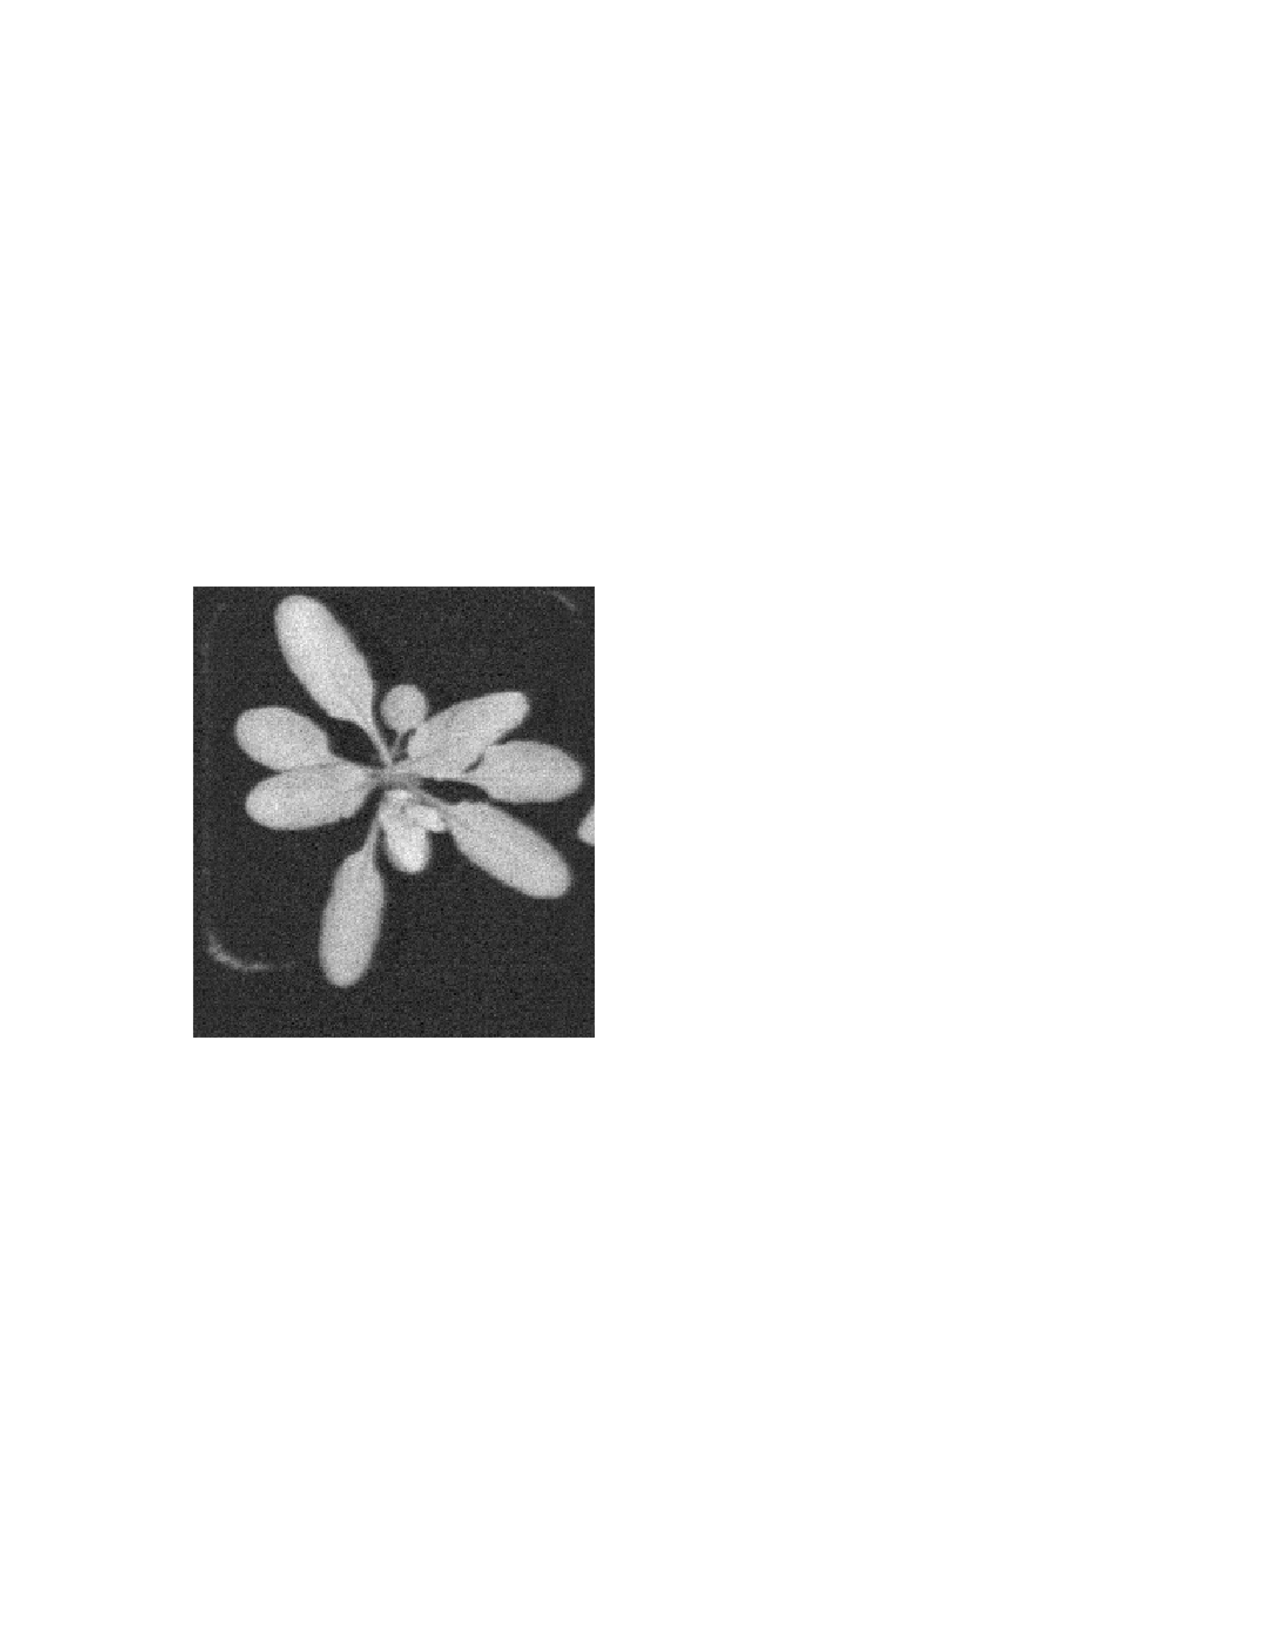
\includegraphics[width=.14\textwidth]{Figures/AlignPerformance/9_1}&
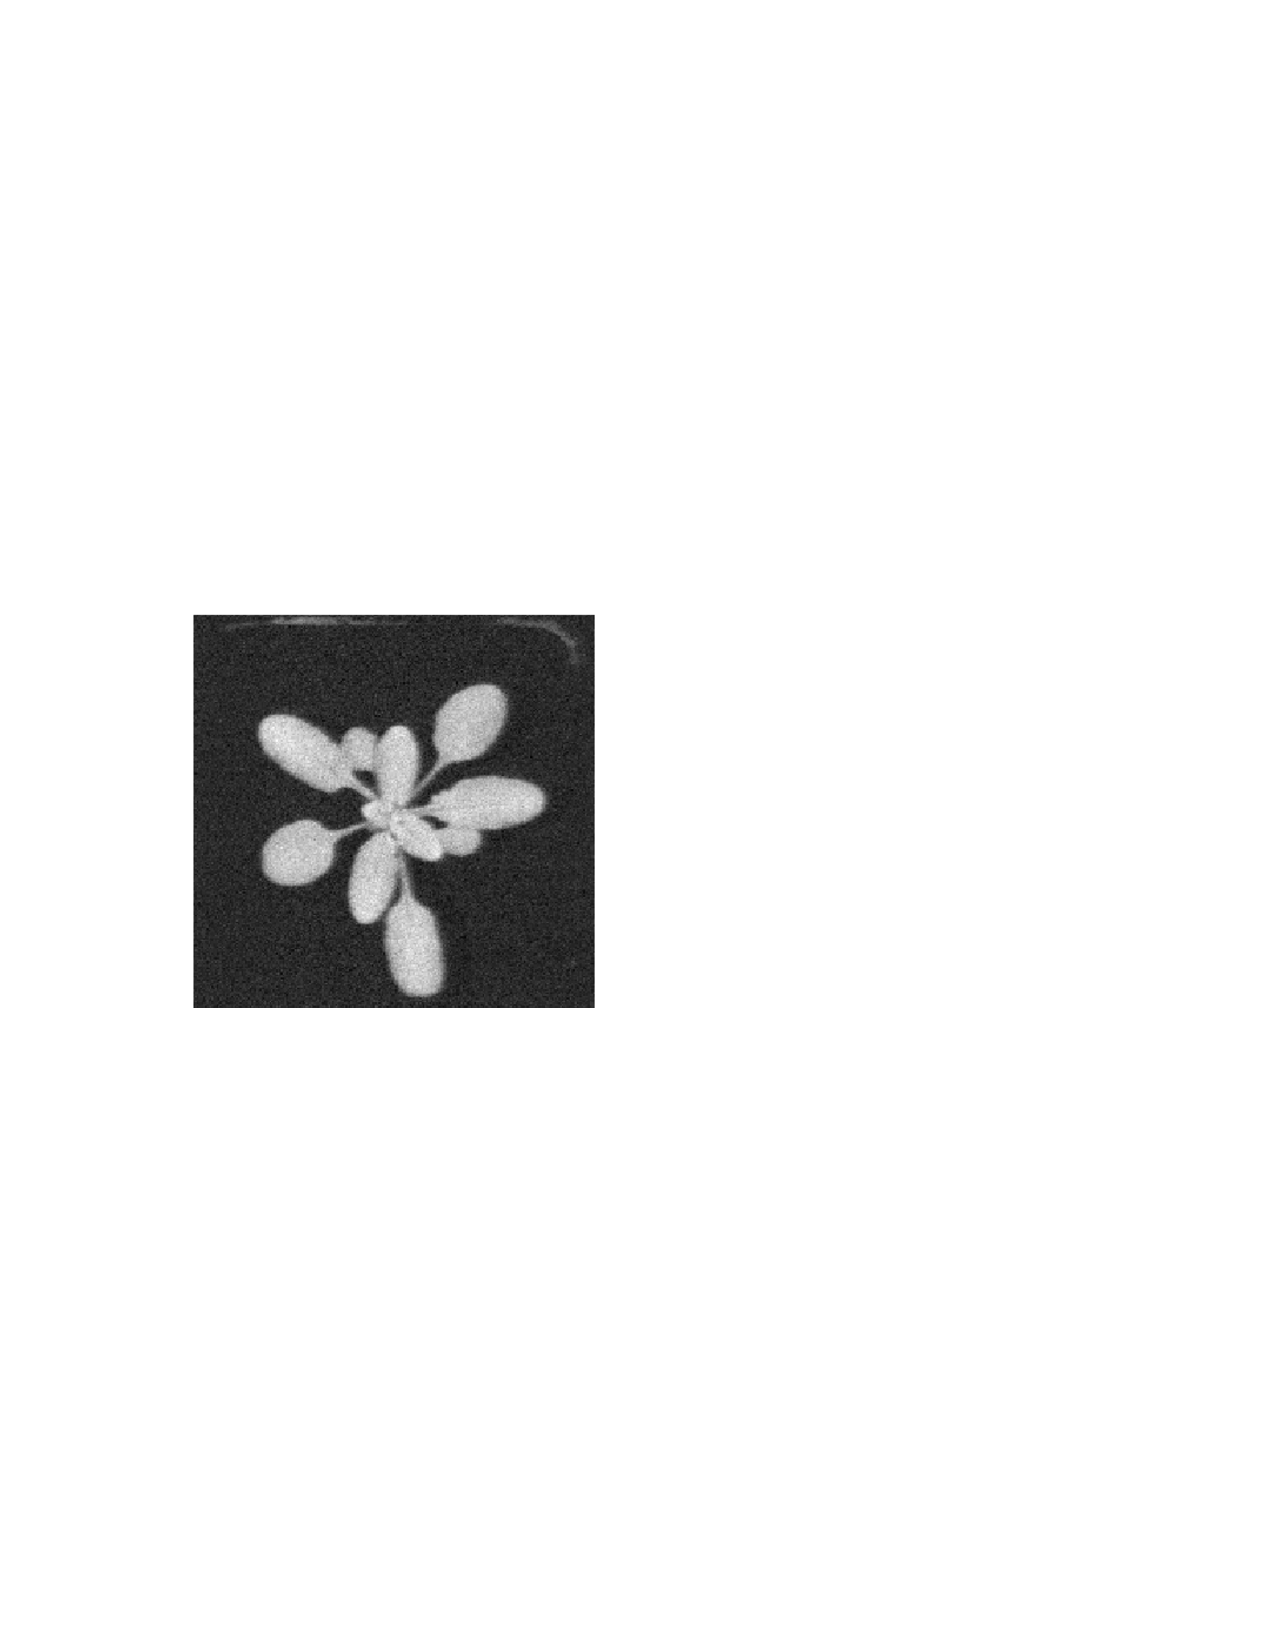
\includegraphics[width=.14\textwidth]{Figures/AlignPerformance/10_1}&
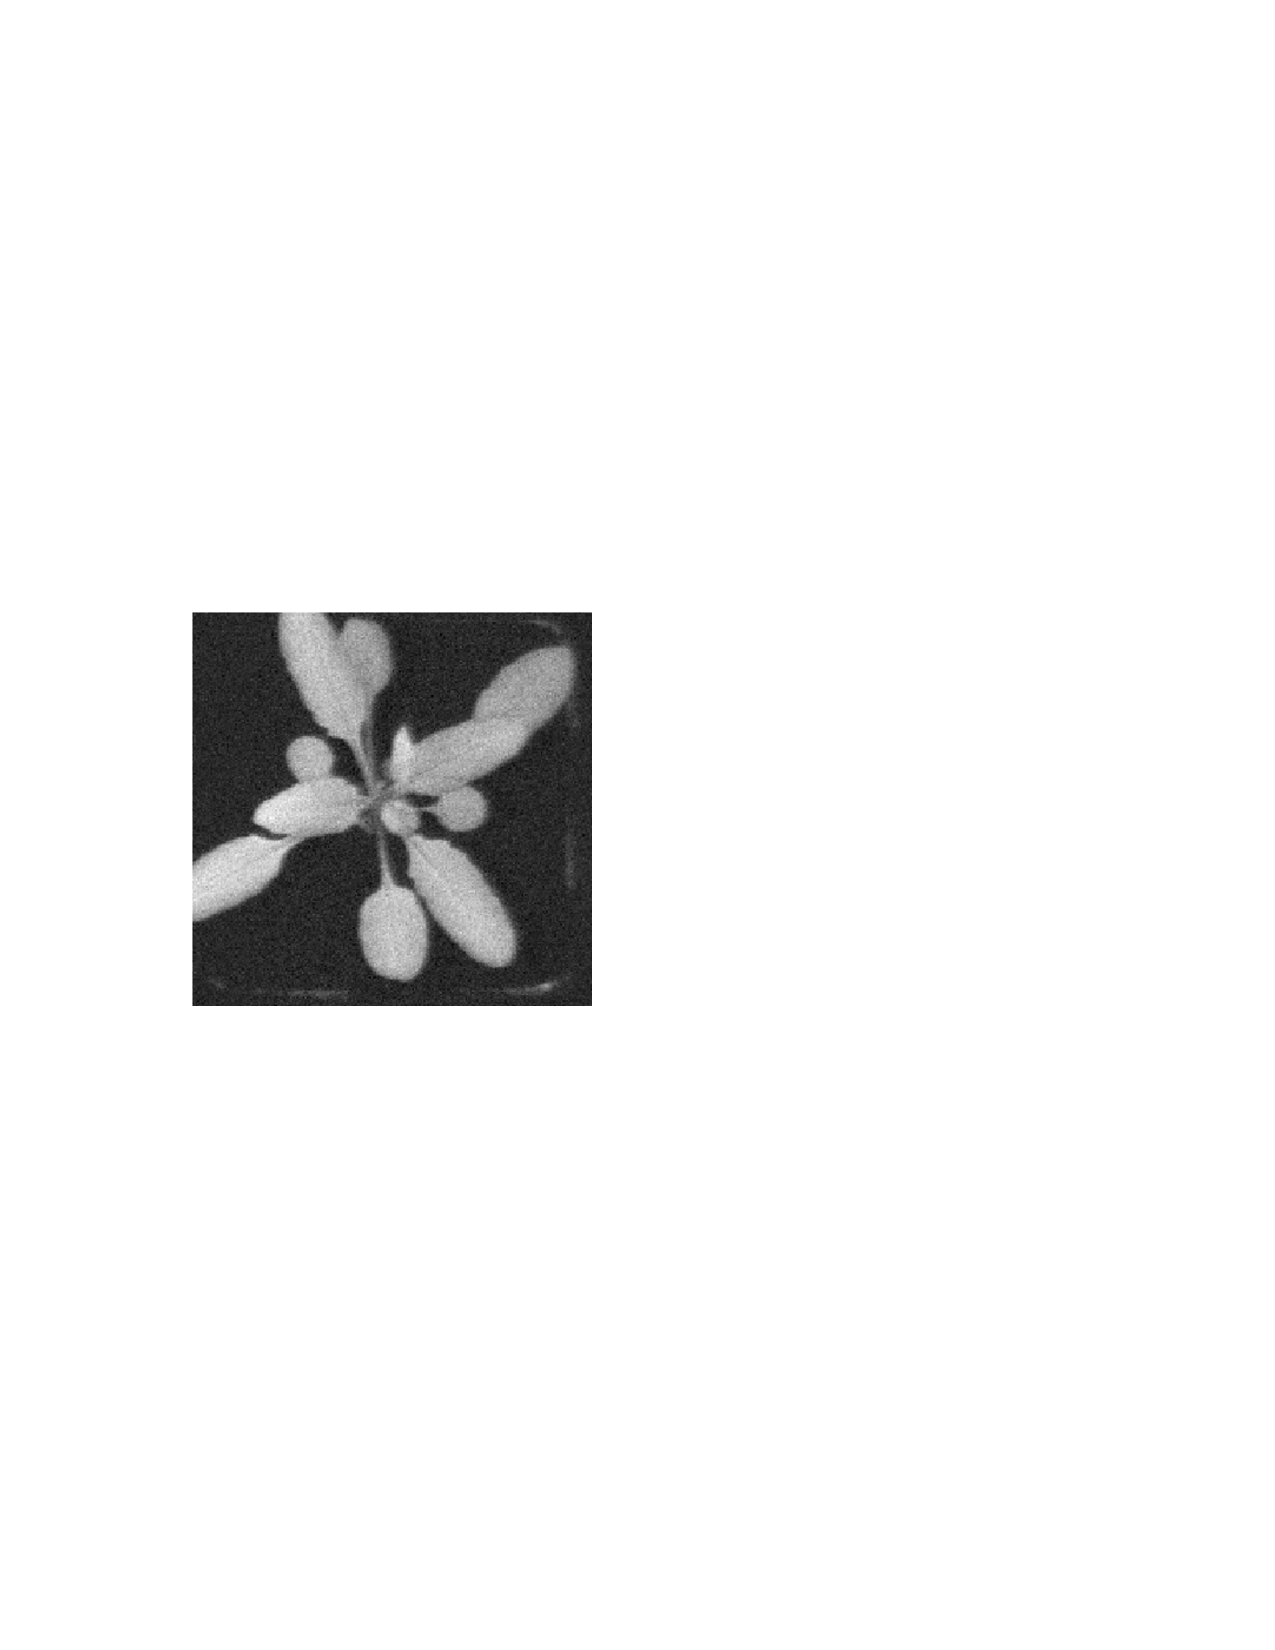
\includegraphics[width=.14\textwidth]{Figures/AlignPerformance/11_1}&
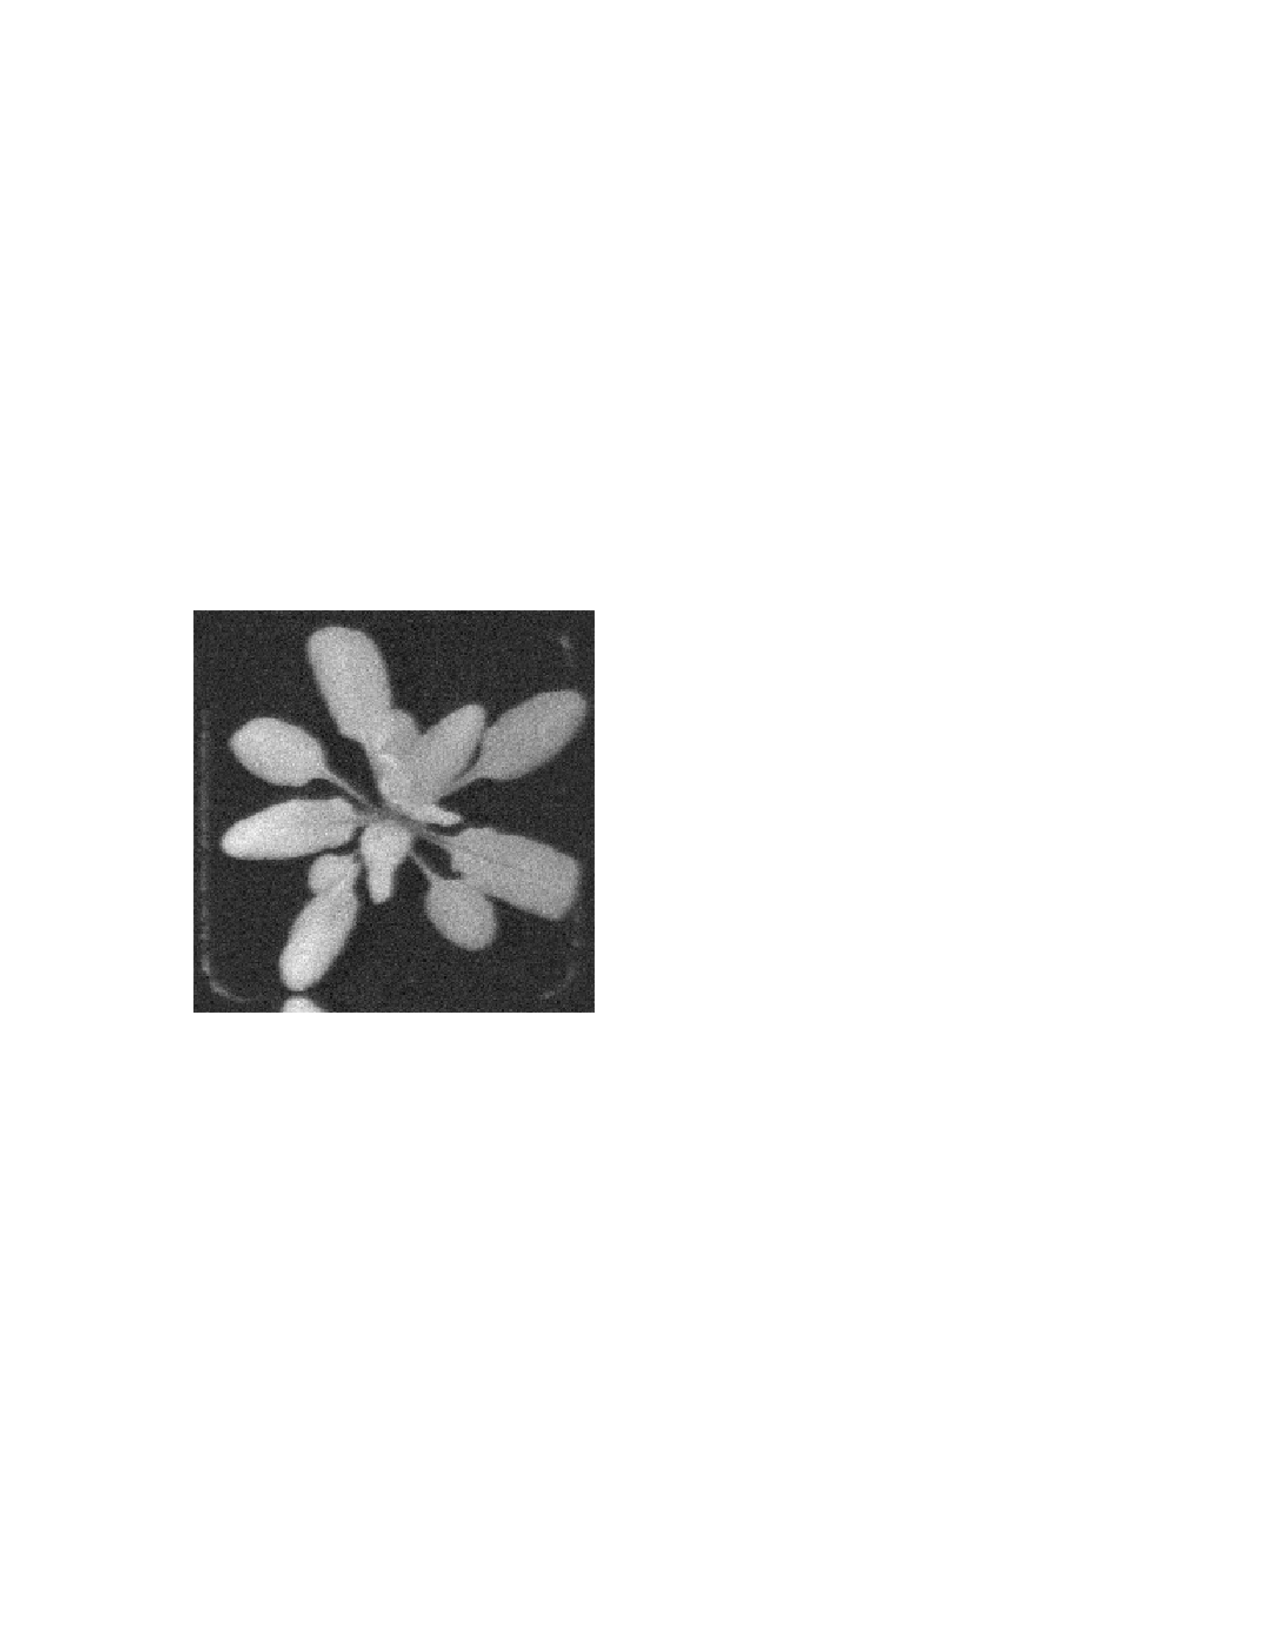
\includegraphics[width=.14\textwidth]{Figures/AlignPerformance/12_1}&
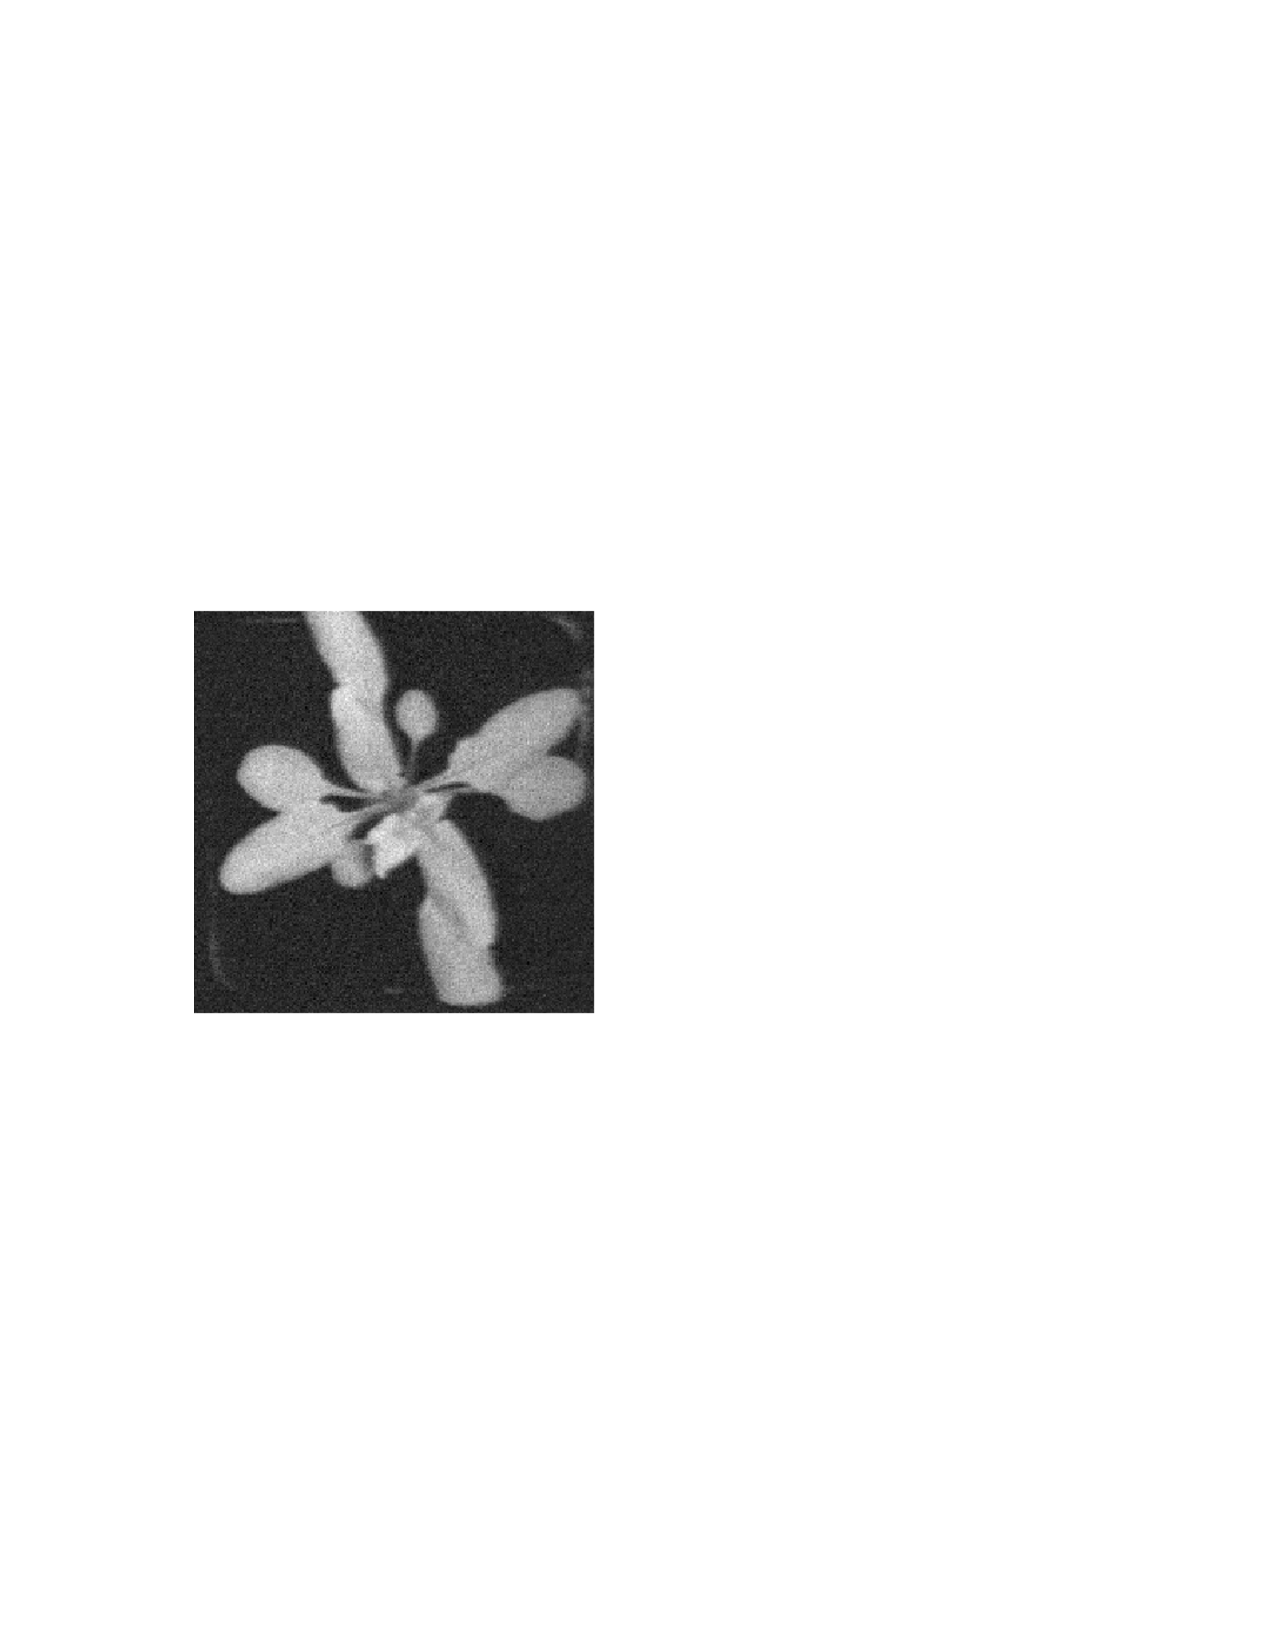
\includegraphics[width=.14\textwidth]{Figures/AlignPerformance/14_1}&
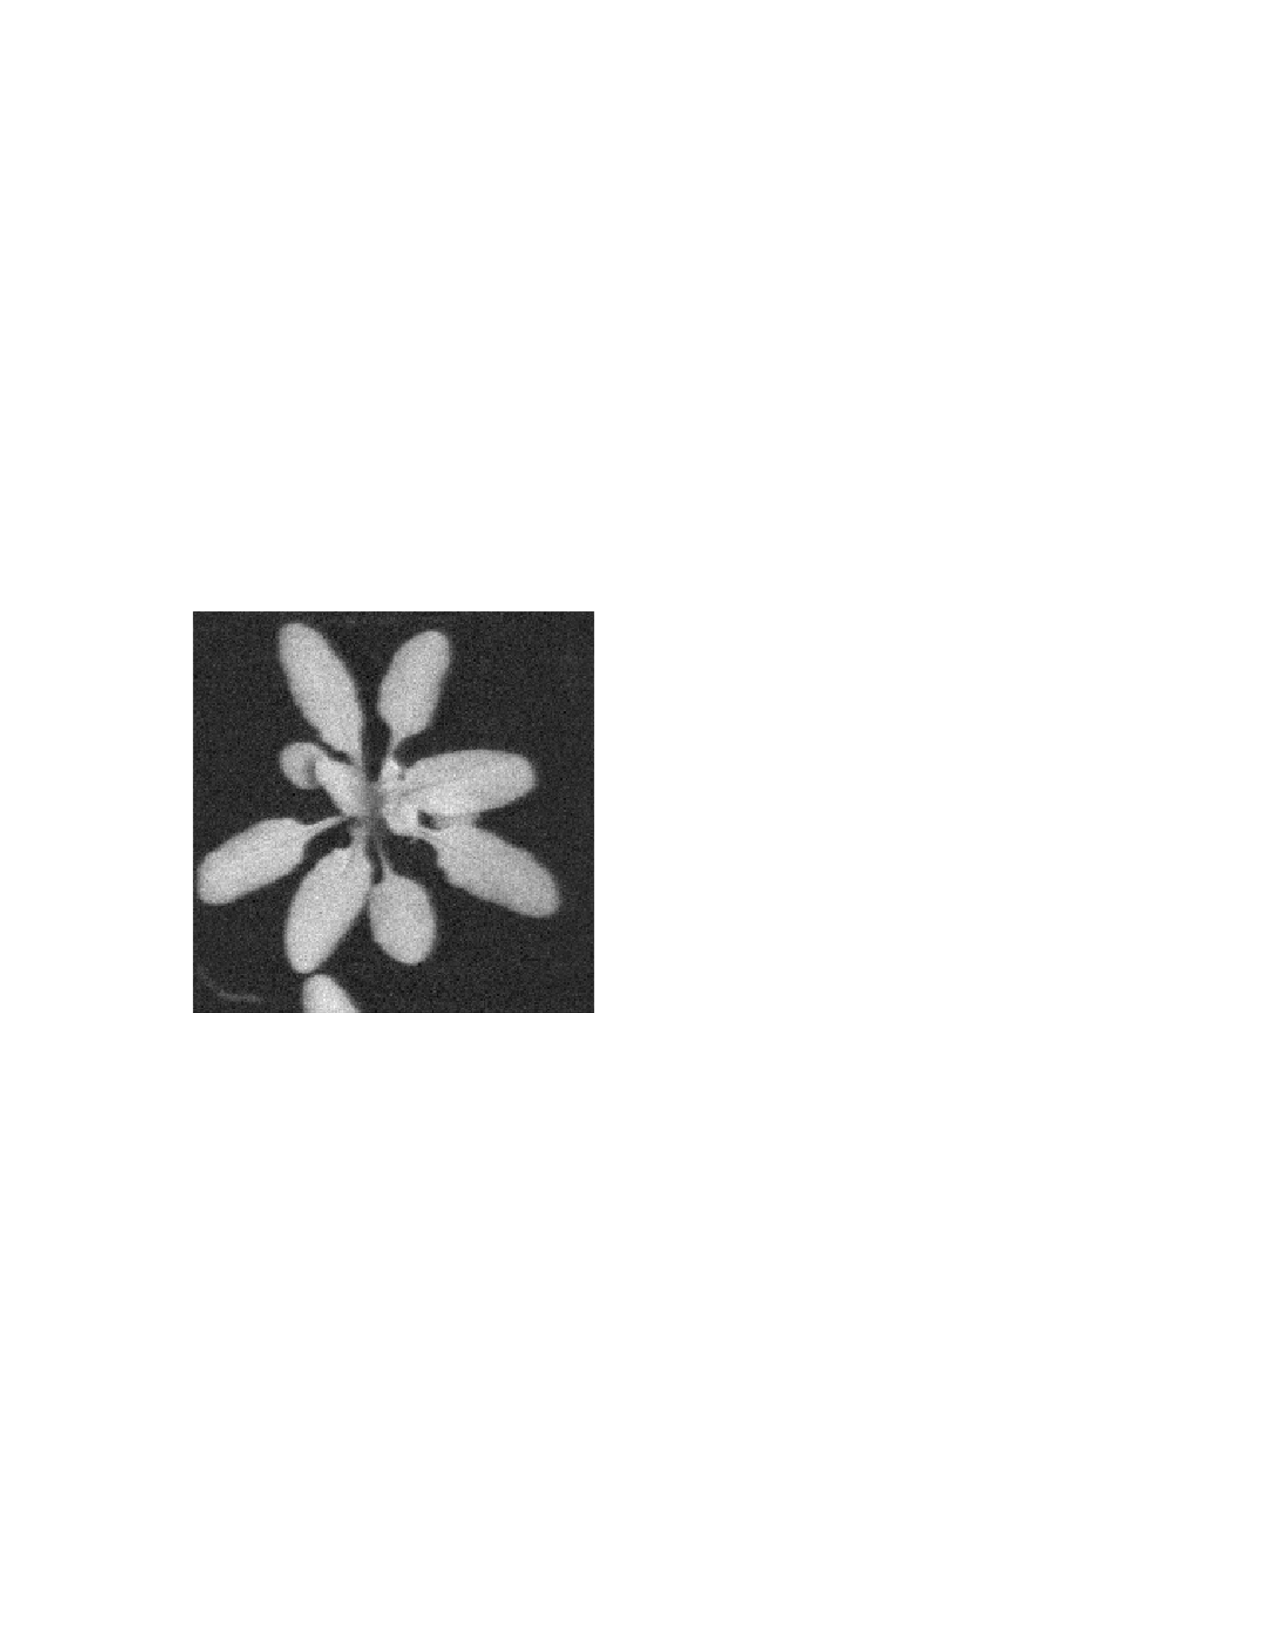
\includegraphics[width=.14\textwidth]{Figures/AlignPerformance/15_1}\\

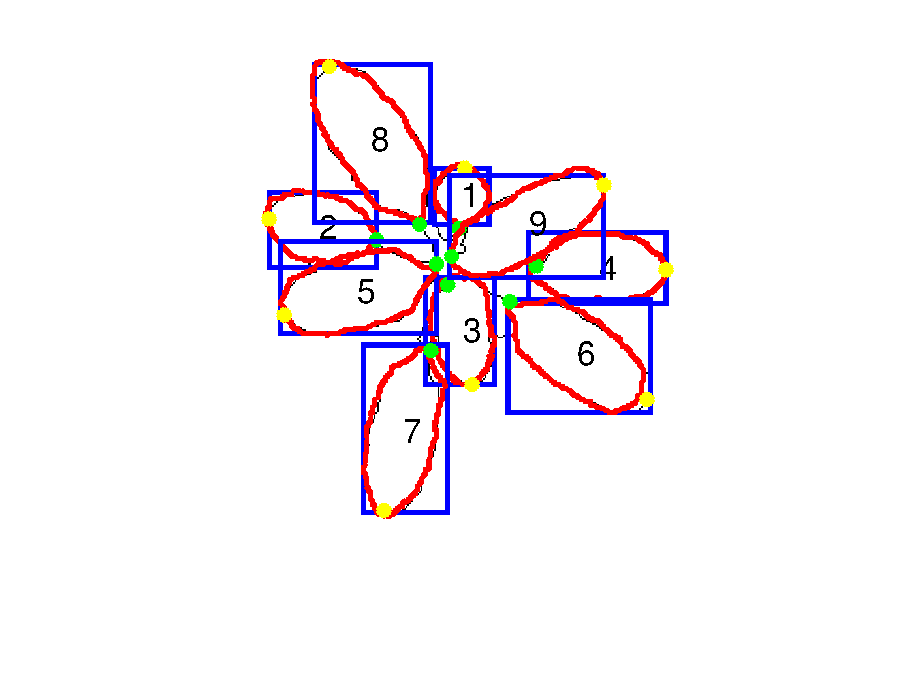
\includegraphics[trim= 90 60 100 5, clip, width=.14\textwidth]{Figures/AlignPerformance/9_2}&
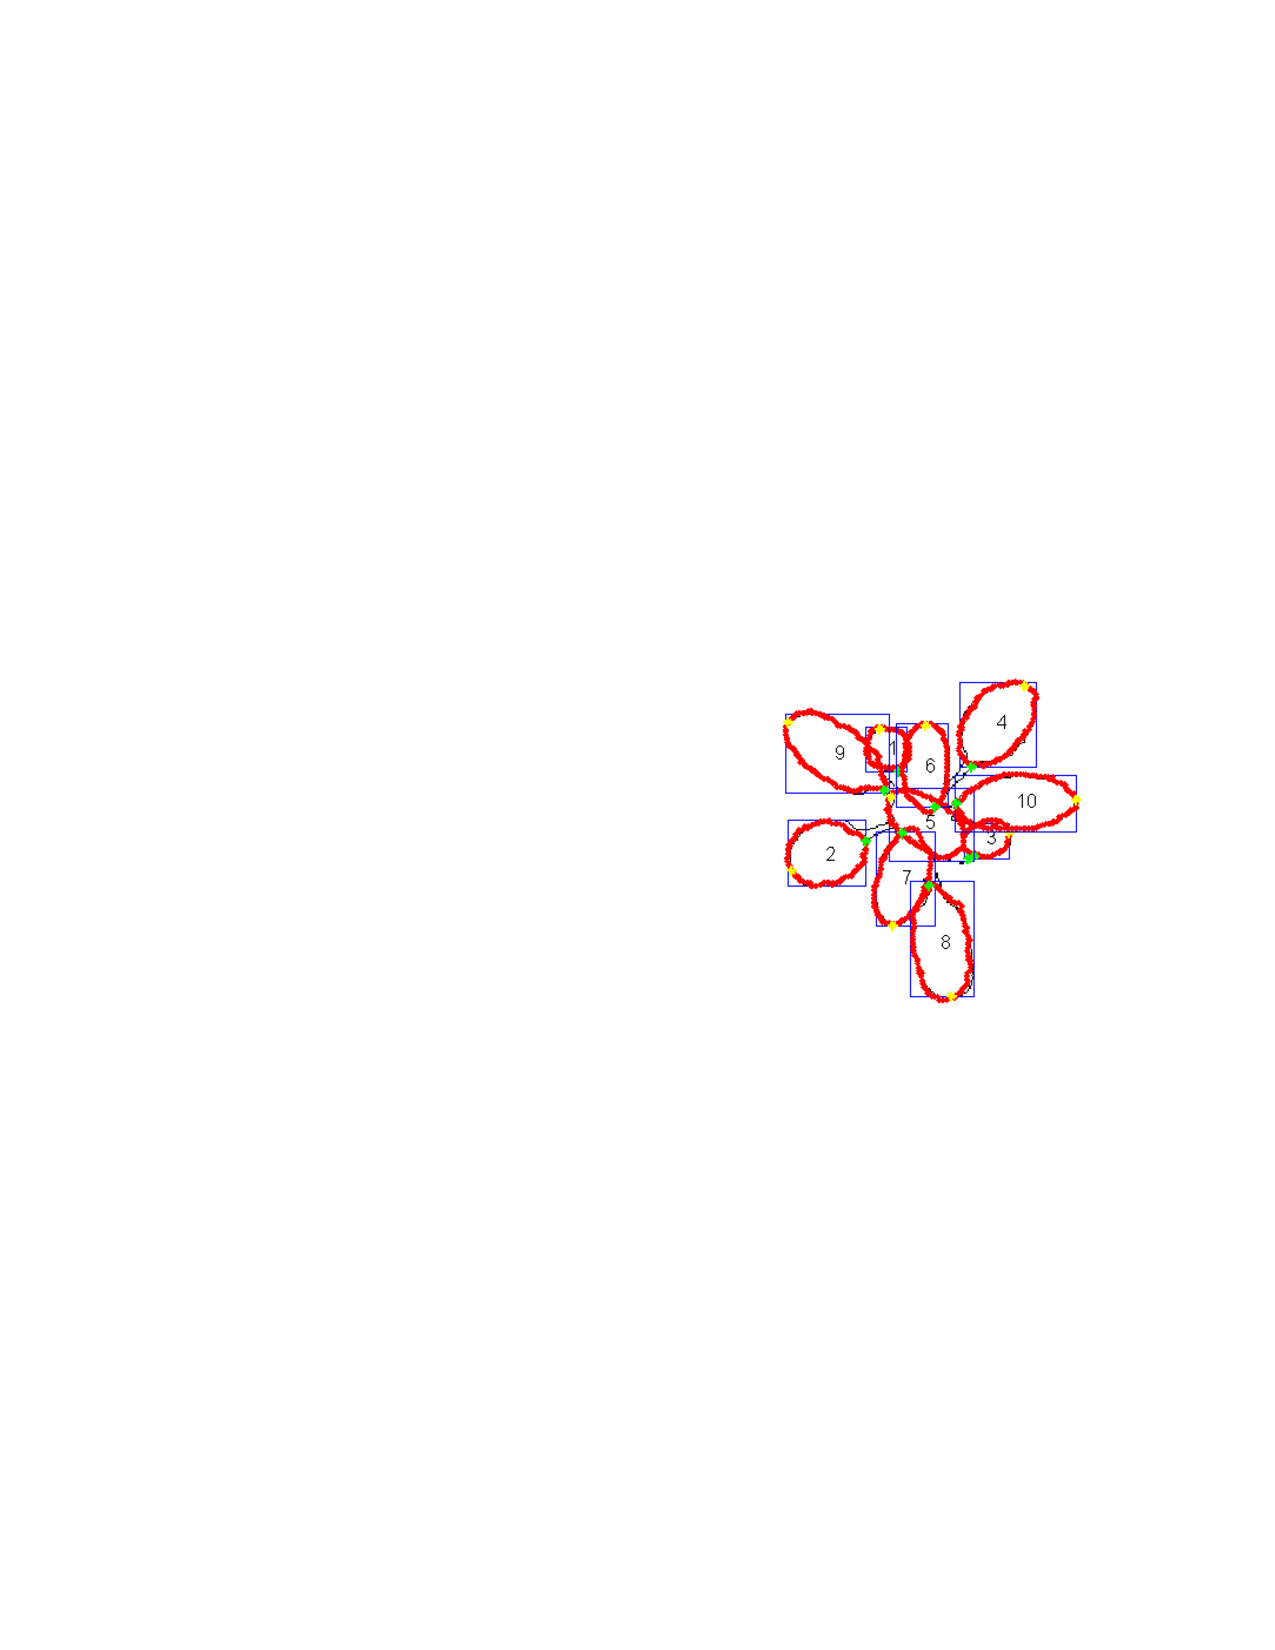
\includegraphics[trim= 90 60 100 5, clip, width=.14\textwidth]{Figures/AlignPerformance/10_2}&
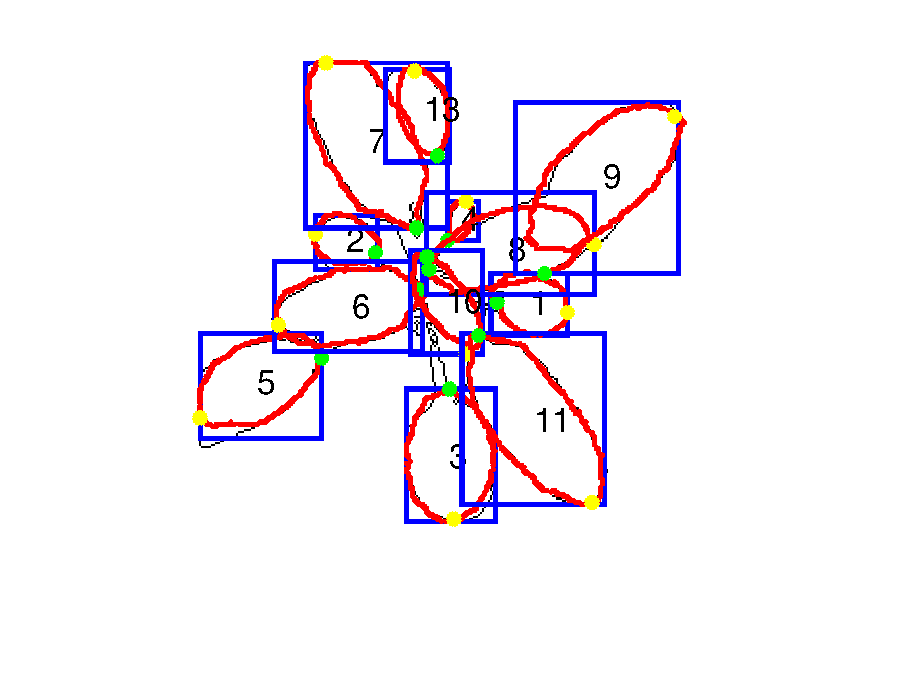
\includegraphics[trim= 90 60 100 5, clip, width=.14\textwidth]{Figures/AlignPerformance/11_2}&
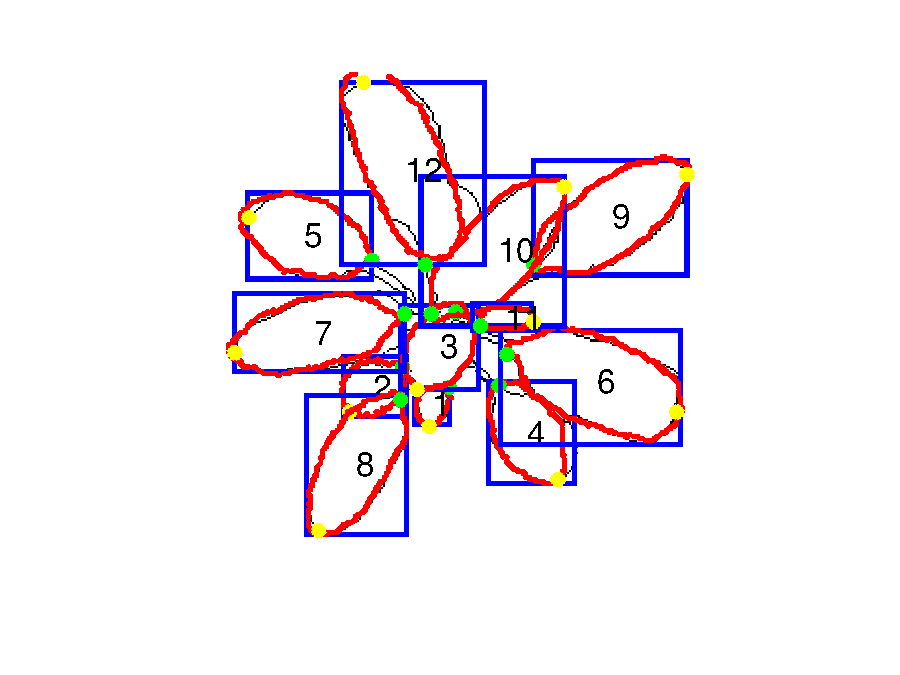
\includegraphics[trim= 90 60 100 5, clip, width=.14\textwidth]{Figures/AlignPerformance/12_2}&
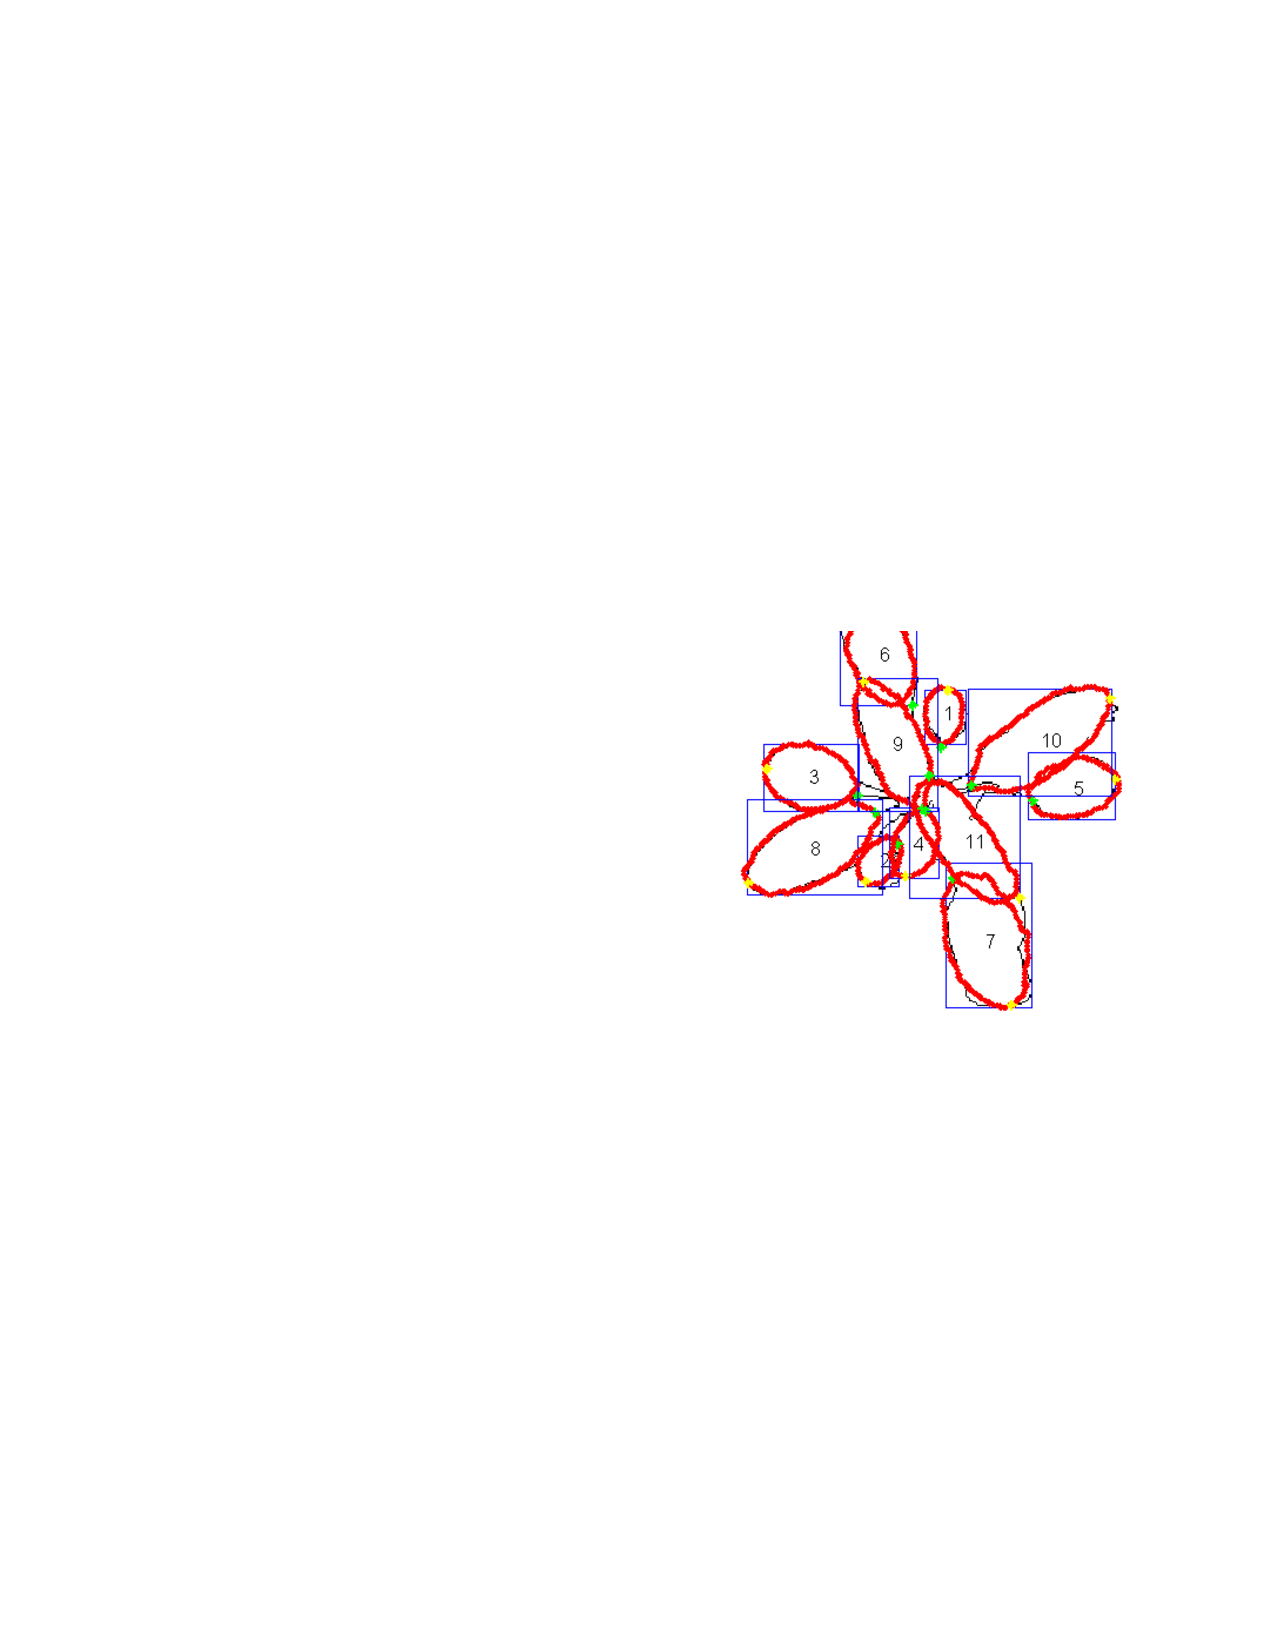
\includegraphics[trim= 90 60 100 5, clip, width=.14\textwidth]{Figures/AlignPerformance/14_2}&
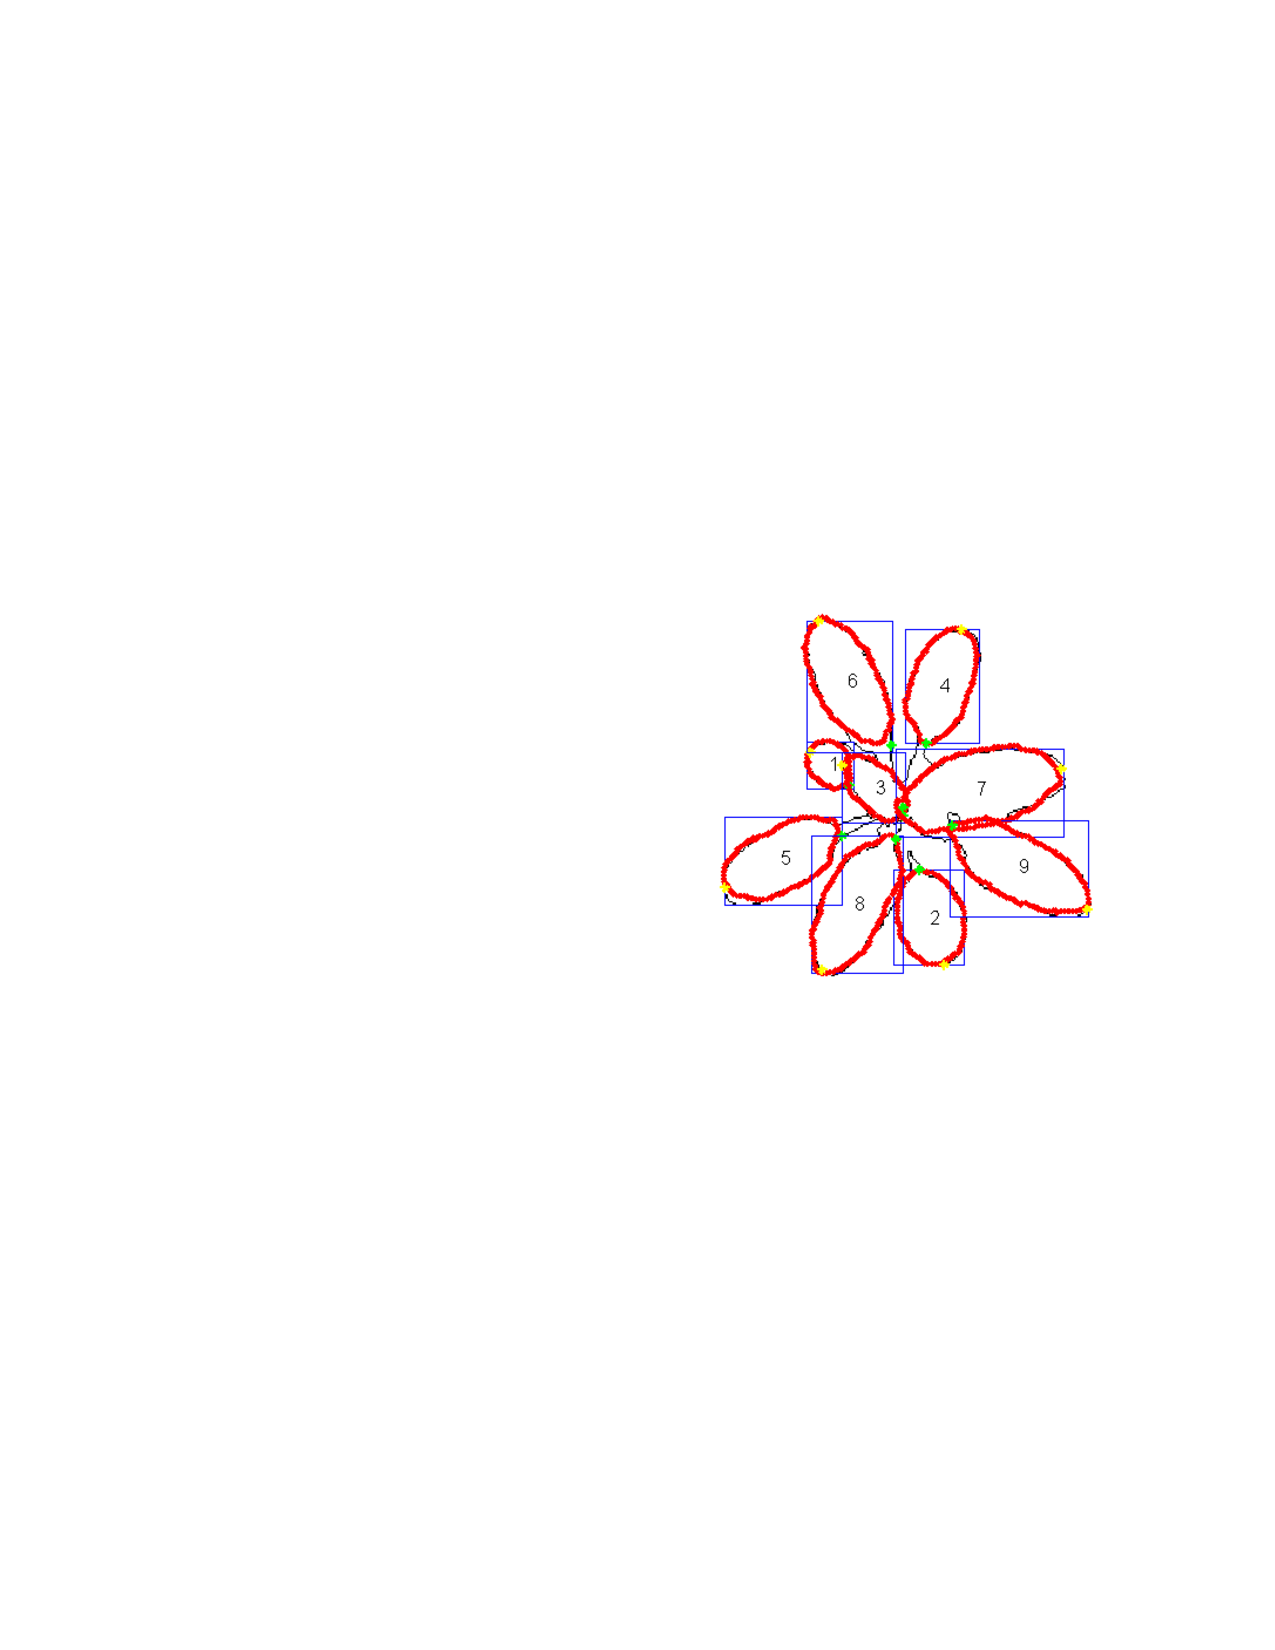
\includegraphics[trim= 90 60 100 5, clip, width=.14\textwidth]{Figures/AlignPerformance/15_2}\\
(a) & (b) & (c) & (d) & (e) & (f) \\
\end{tabular}
\caption{Leaf alignment results on the last frame of $6$ plant videos. First row shows the original images. Second row shows the alignment results with red points denoting the boundary of the leaf templates in the blue bounding boxes. The numbers on the leaves are the leaf IDs representing the order of the leaf being selected and they will be consistent during tracking.}
\label{fig:alignResult}
\end{centering}
\end{figure*}



\begin{figure*}
\begin{centering}
\begin{tabular}{c c@{} c@{} c@{} c@{} c@{} c@{} c@{} c@{} c@{}}
%\begin{tabular}{lllllllll}
(a) &
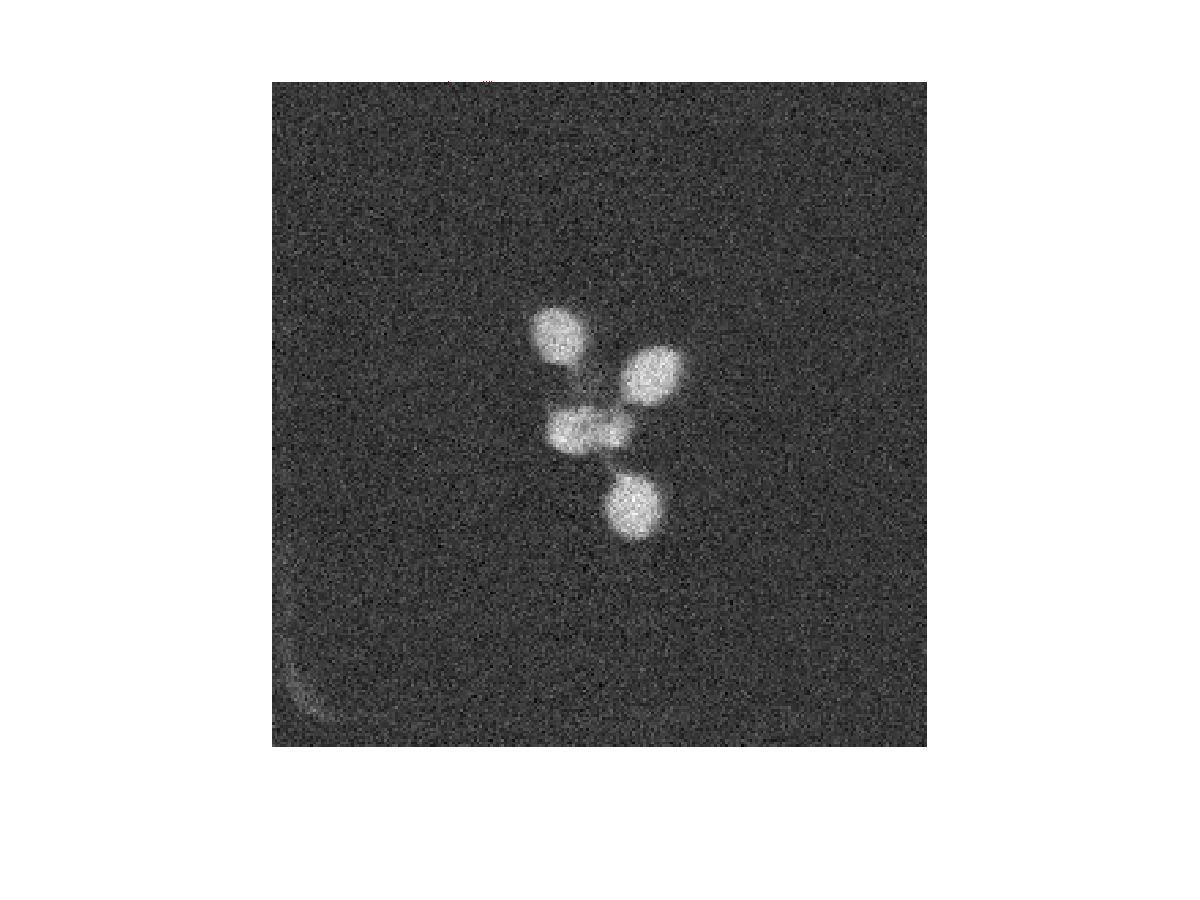
\includegraphics[trim= 100 100 150 10, clip, width=.1\textwidth]{Figures/trackExample/1_1}&
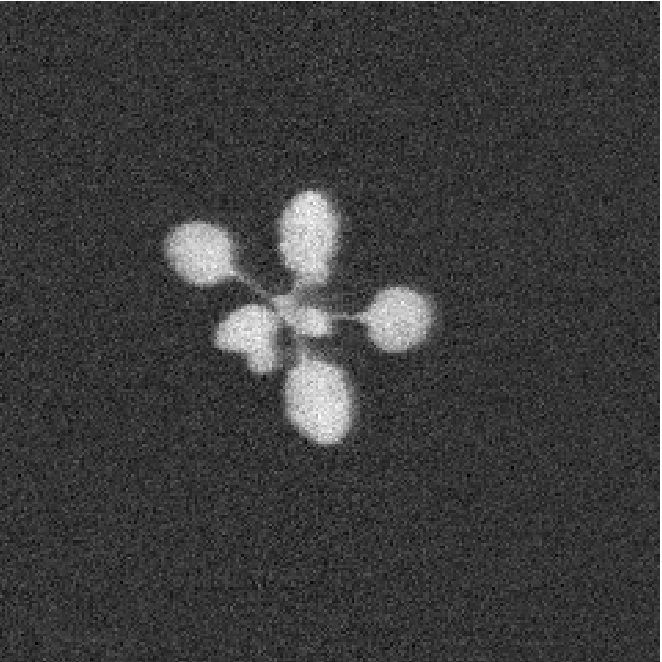
\includegraphics[trim= 100 100 150 10, clip, width=.1\textwidth]{Figures/trackExample/1_2}&
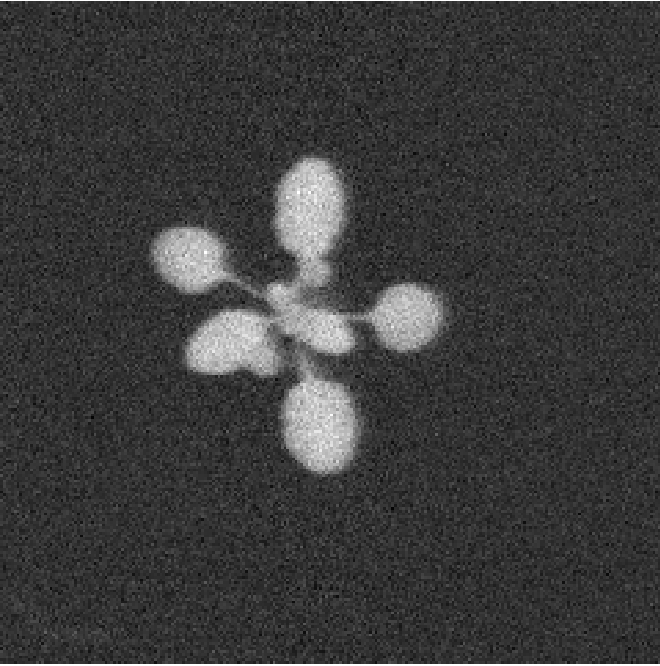
\includegraphics[trim= 100 100 150 10, clip, width=.1\textwidth]{Figures/trackExample/1_3}&
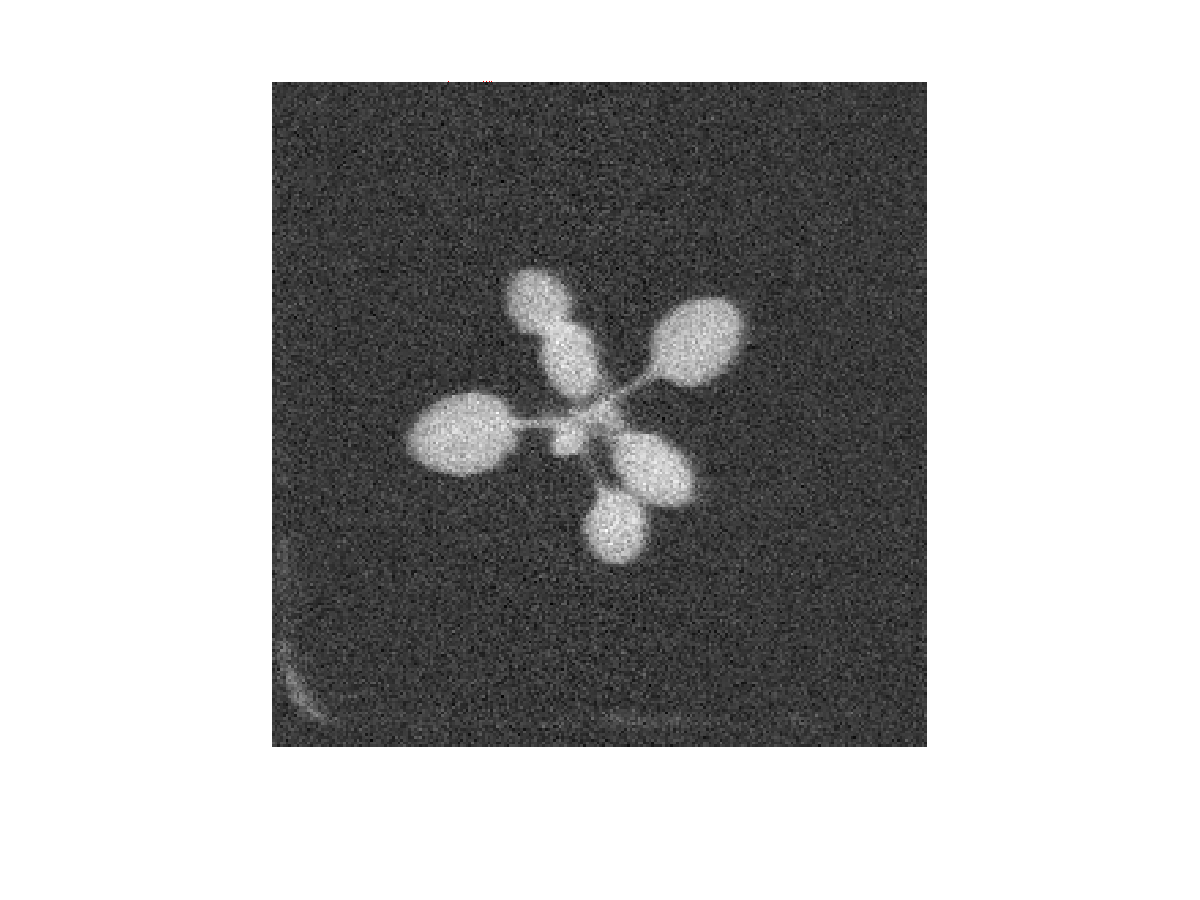
\includegraphics[trim= 100 100 150 10, clip, width=.1\textwidth]{Figures/trackExample/1_4}&
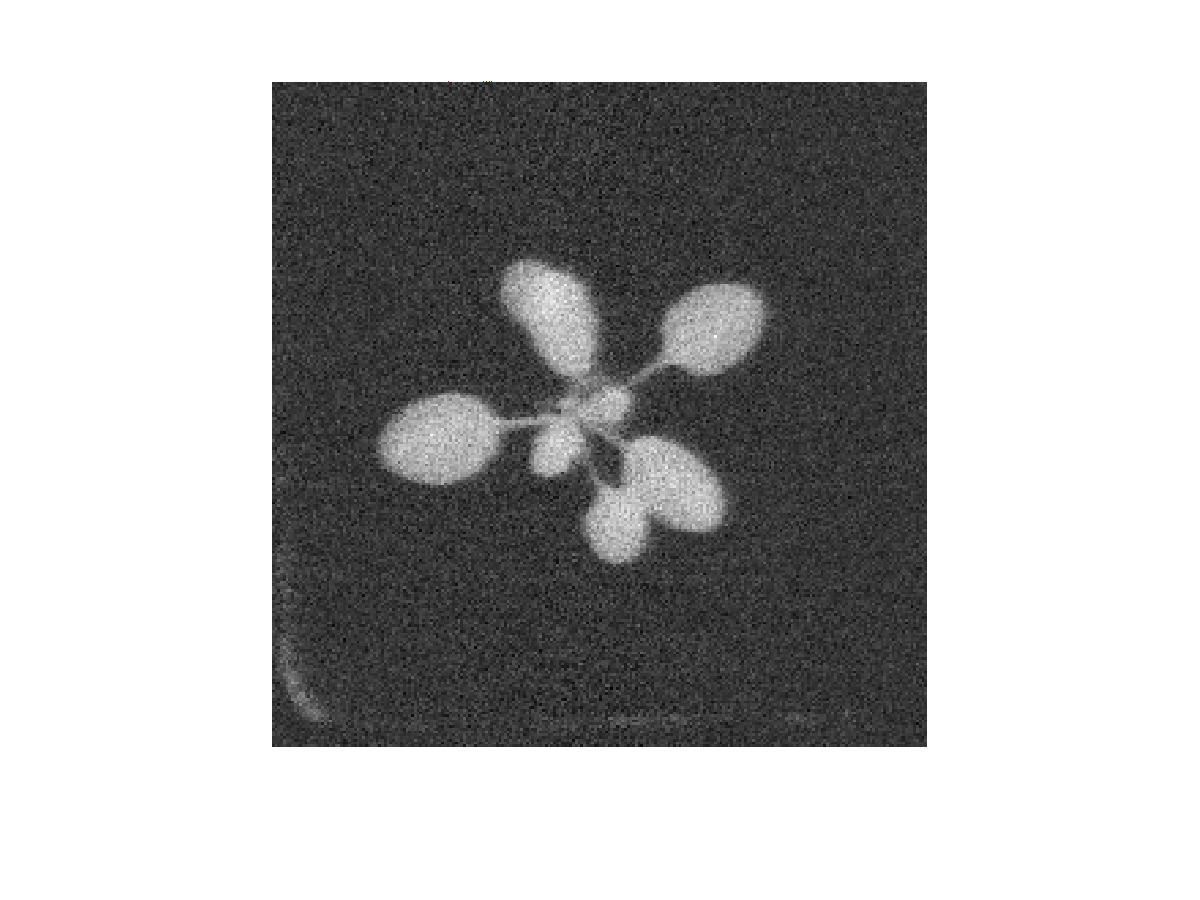
\includegraphics[trim= 100 100 150 10, clip, width=.1\textwidth]{Figures/trackExample/1_5}&
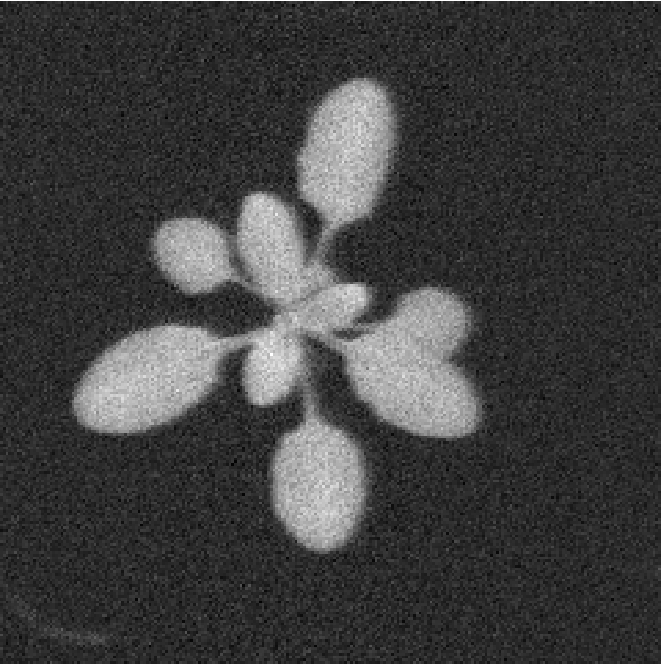
\includegraphics[trim= 100 100 150 10, clip, width=.1\textwidth]{Figures/trackExample/1_6}&
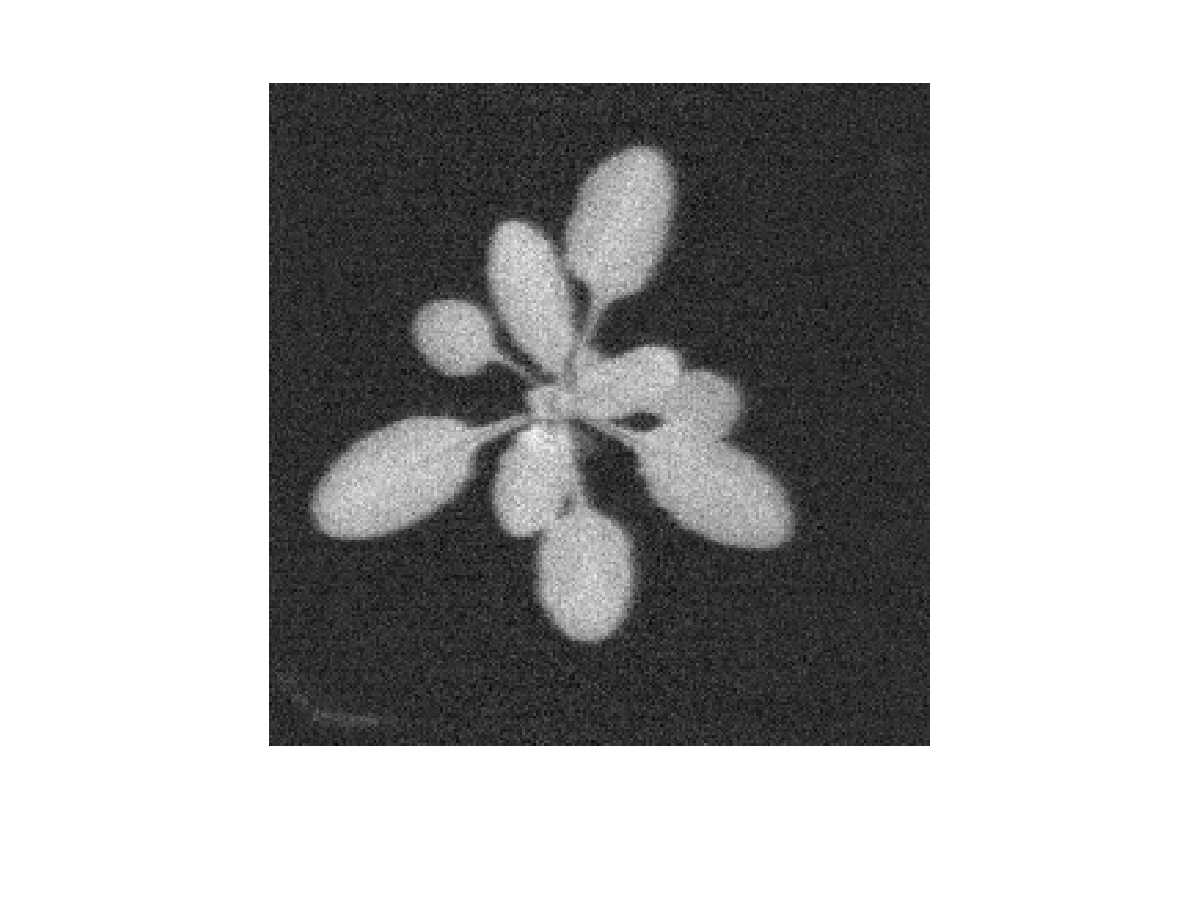
\includegraphics[trim= 100 100 150 10, clip, width=.1\textwidth]{Figures/trackExample/1_7}&
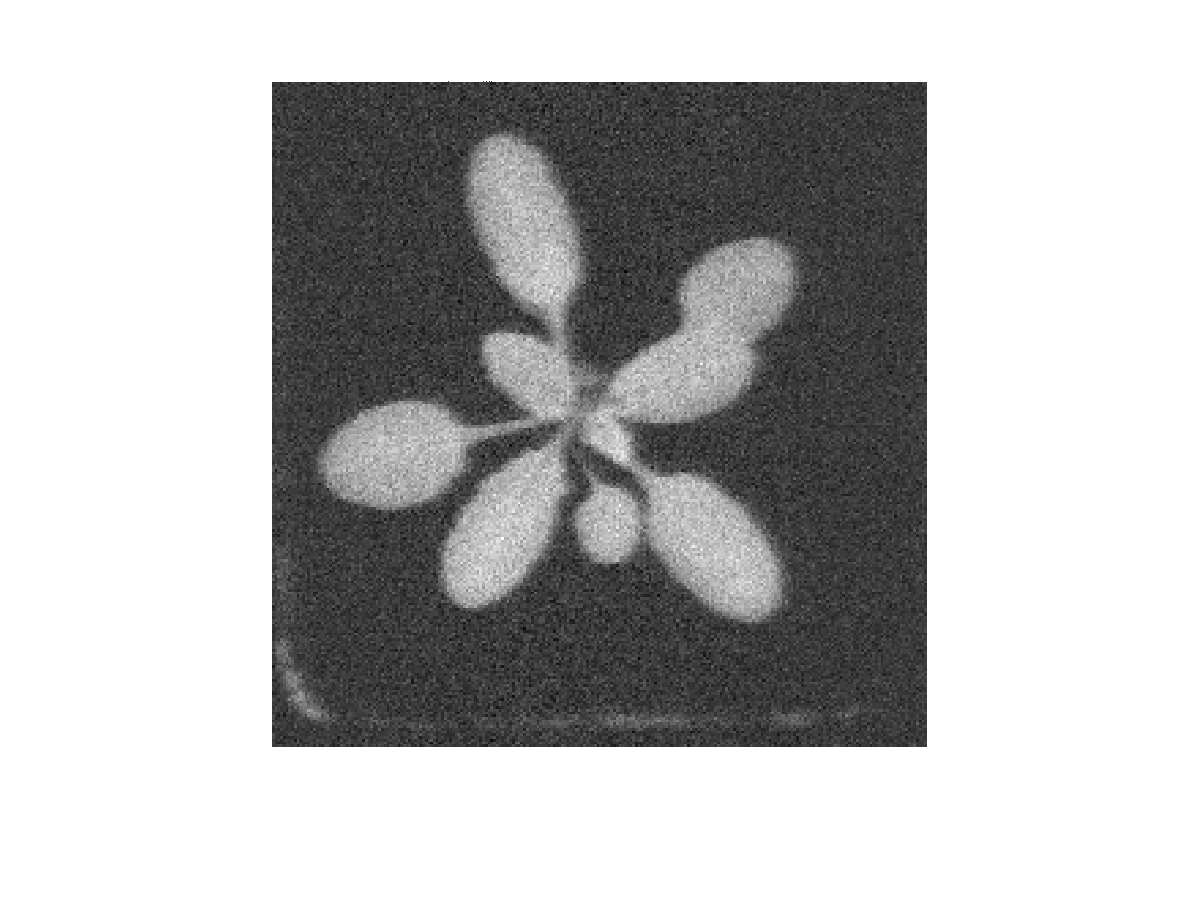
\includegraphics[trim= 100 100 150 10, clip, width=.1\textwidth]{Figures/trackExample/1_8}&
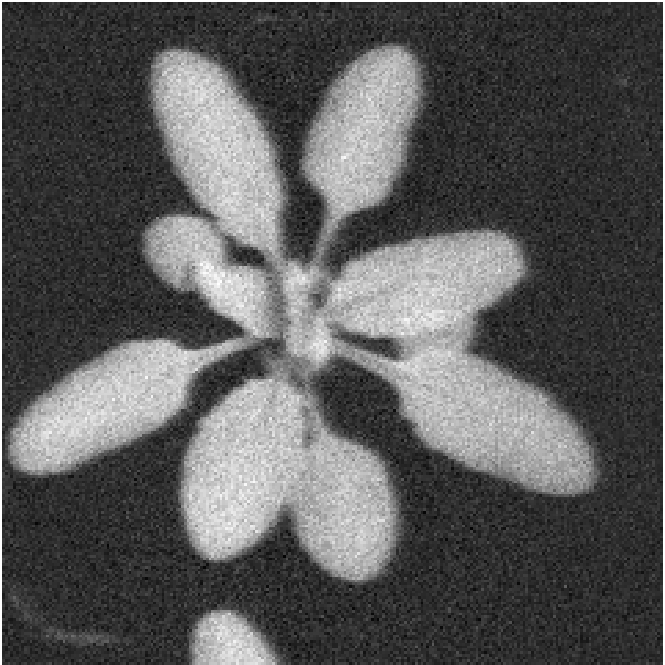
\includegraphics[trim= 100 100 150 10, clip, width=.1\textwidth]{Figures/trackExample/1_9}\\
(b)&
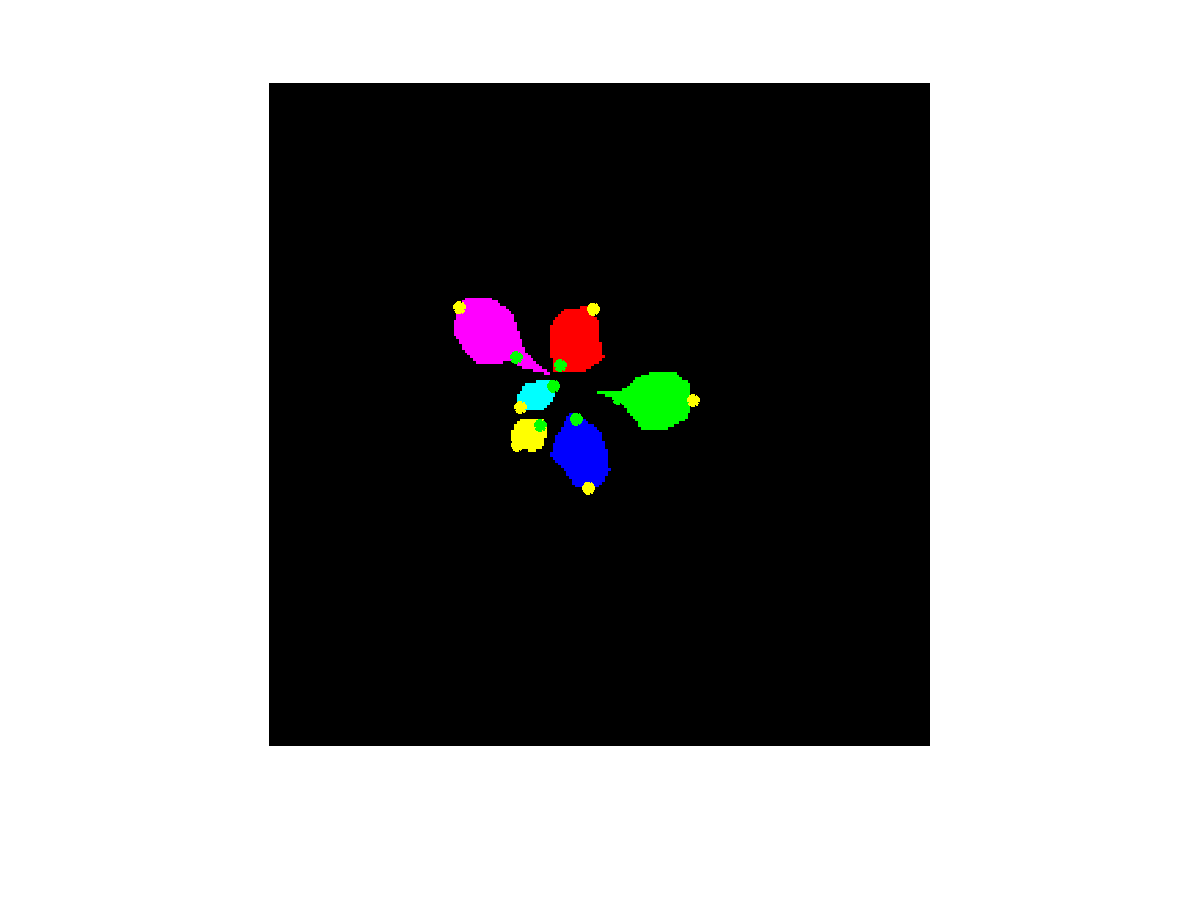
\includegraphics[trim= 100 100 150 10, clip, width=.1\textwidth]{Figures/trackExample/2_1}&
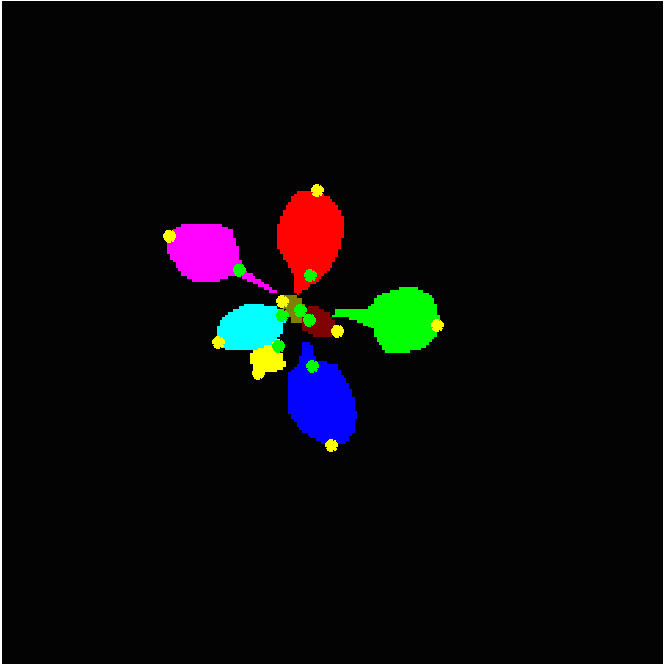
\includegraphics[trim= 100 100 150 10, clip, width=.1\textwidth]{Figures/trackExample/2_2}&
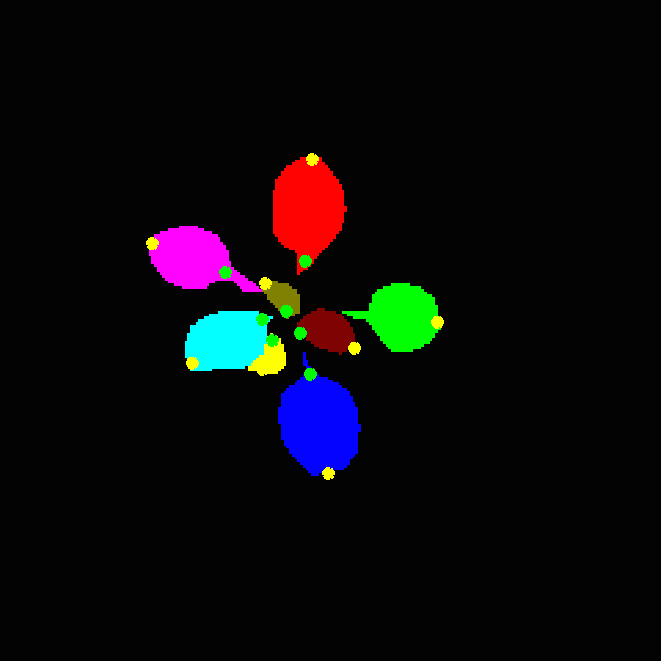
\includegraphics[trim= 100 100 150 10, clip, width=.1\textwidth]{Figures/trackExample/2_3}&
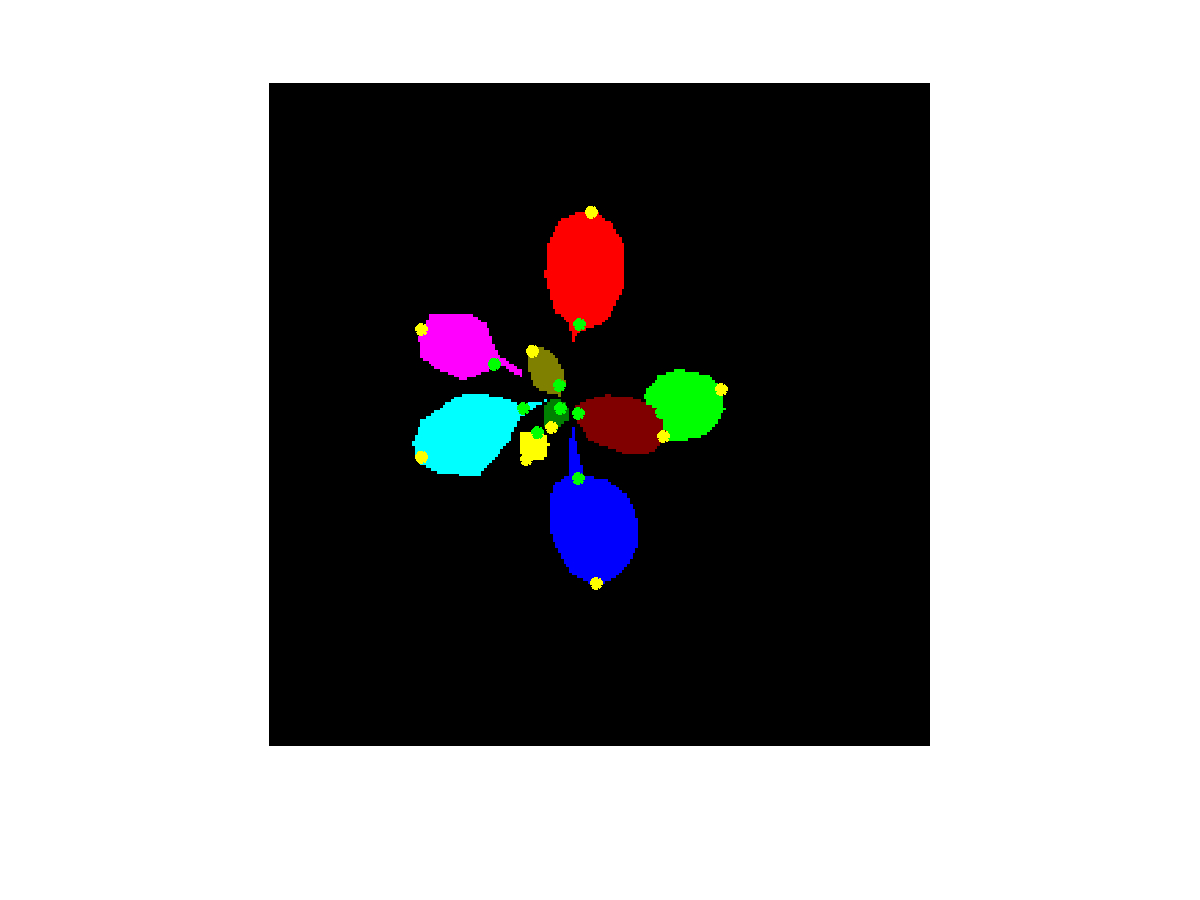
\includegraphics[trim= 100 100 150 10, clip, width=.1\textwidth]{Figures/trackExample/2_4}&
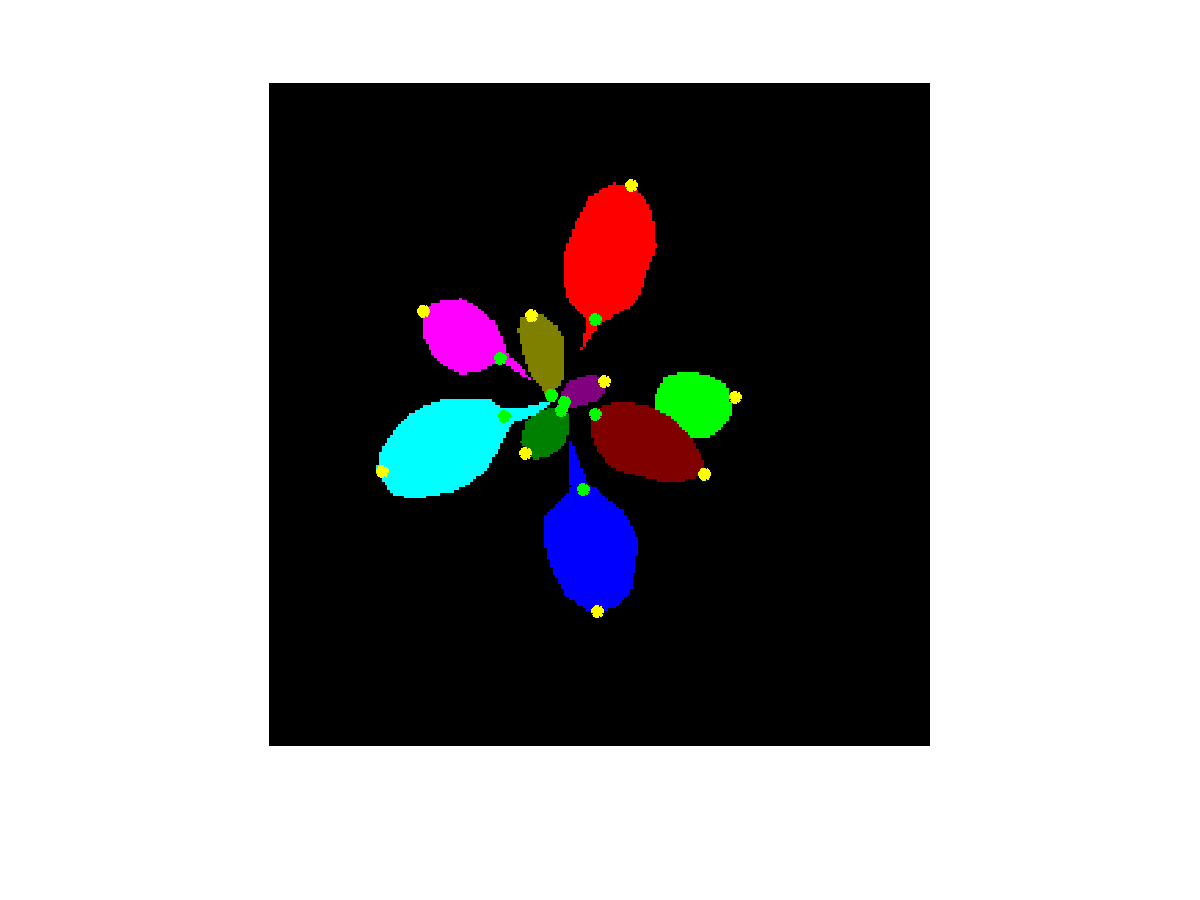
\includegraphics[trim= 100 100 150 10, clip, width=.1\textwidth]{Figures/trackExample/2_5}&
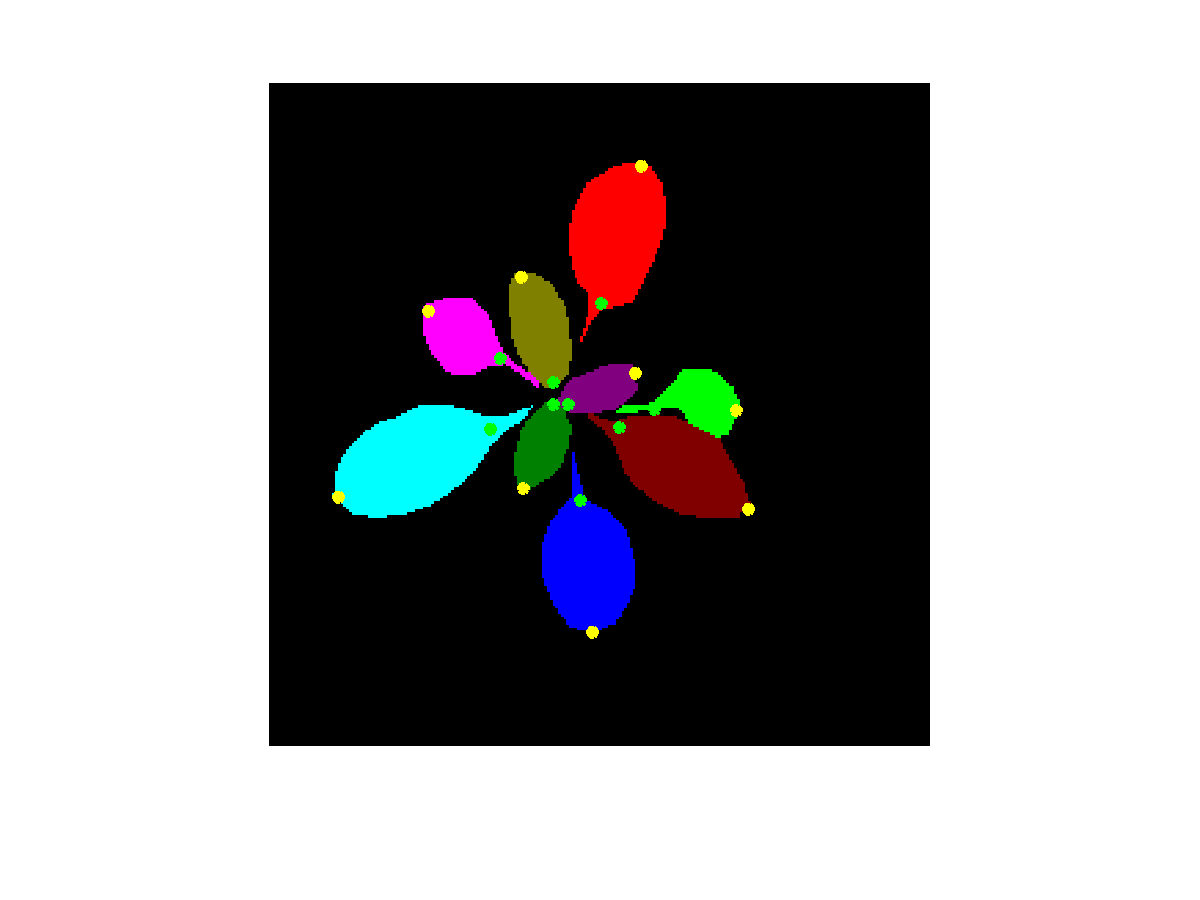
\includegraphics[trim= 100 100 150 10, clip, width=.1\textwidth]{Figures/trackExample/2_6}&
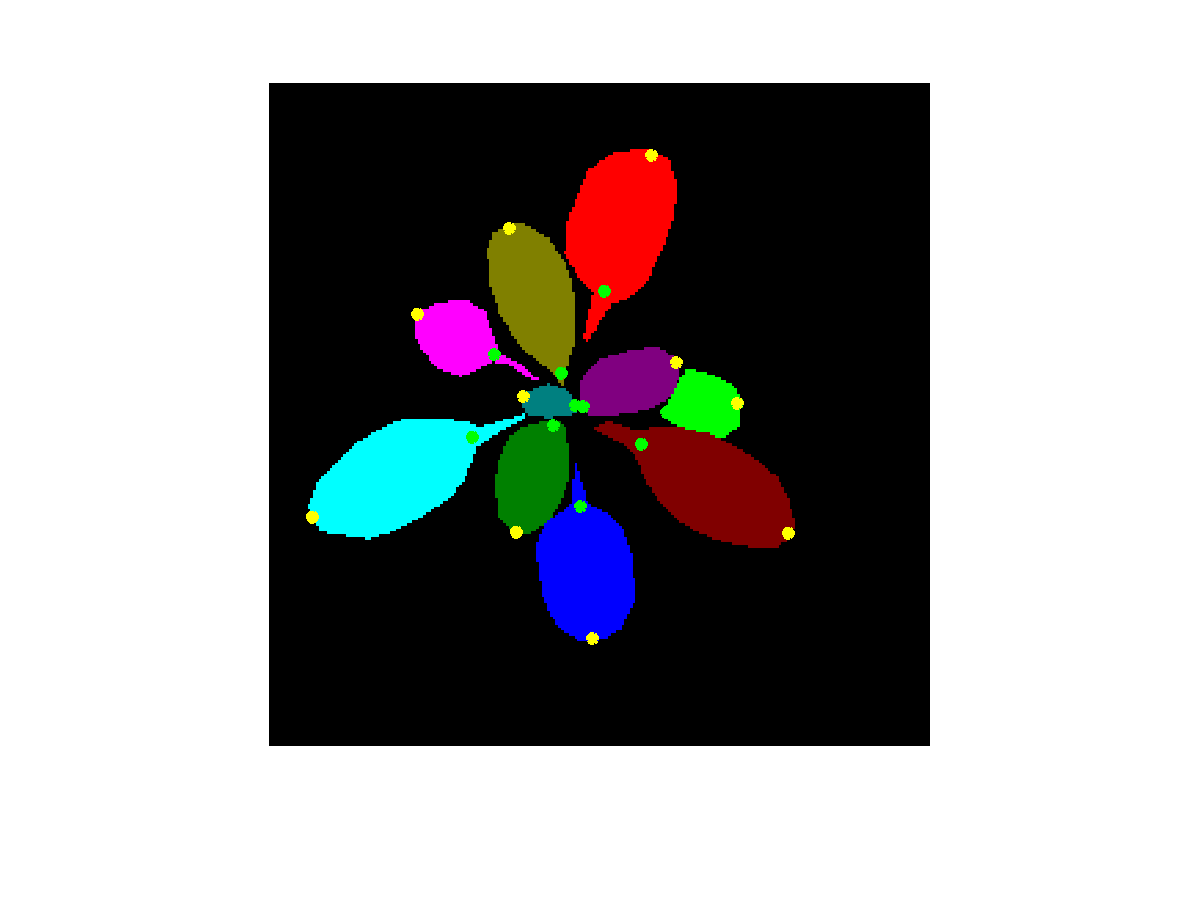
\includegraphics[trim= 100 100 150 10, clip, width=.1\textwidth]{Figures/trackExample/2_7}&
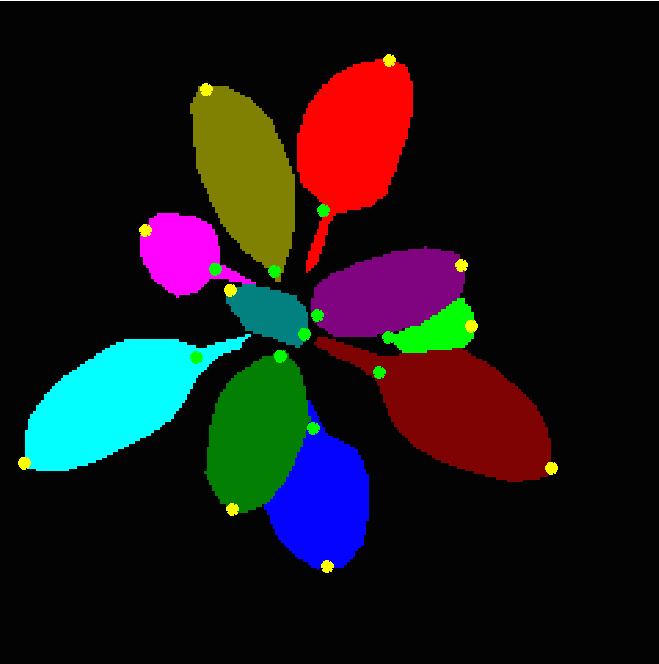
\includegraphics[trim= 100 100 150 10, clip, width=.1\textwidth]{Figures/trackExample/2_8}&
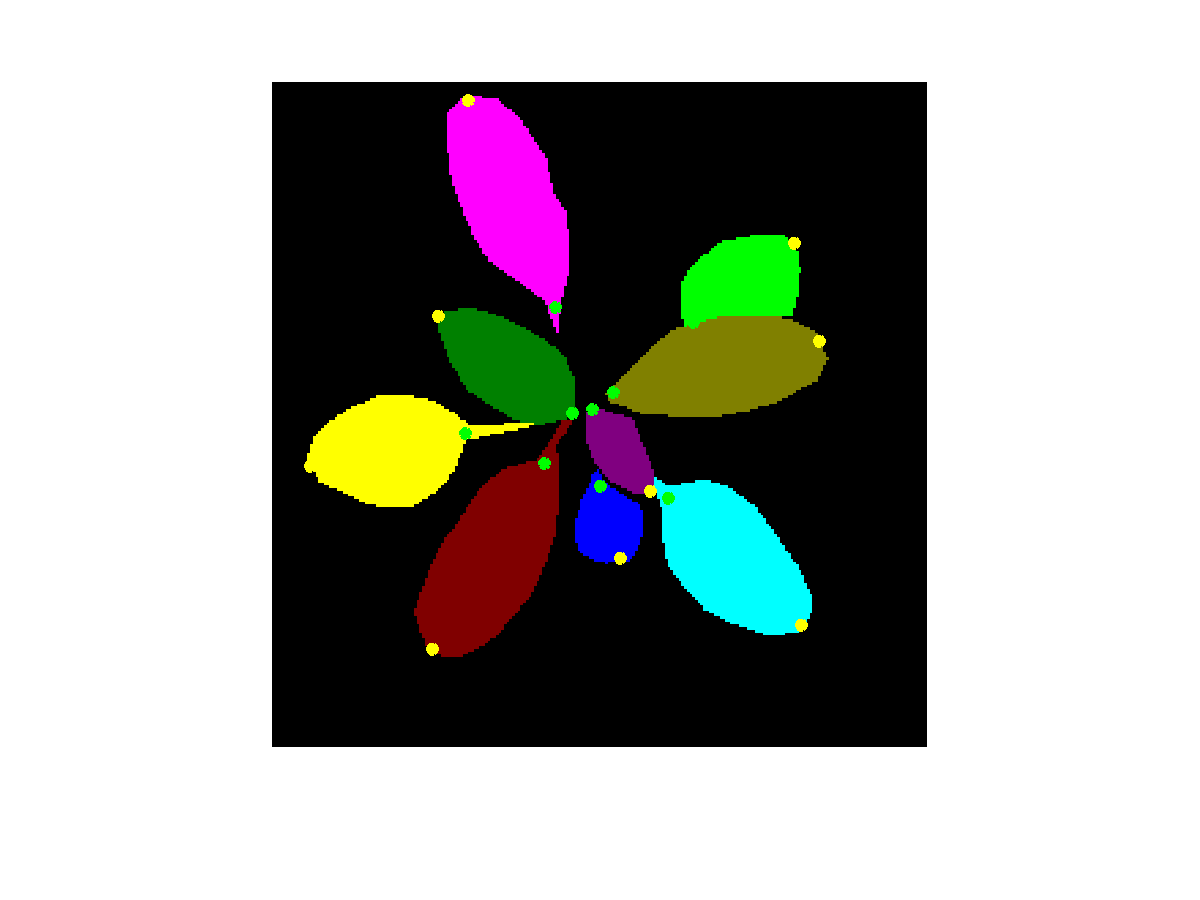
\includegraphics[trim= 100 100 150 10, clip, width=.1\textwidth]{Figures/trackExample/2_9}\\
(c) &
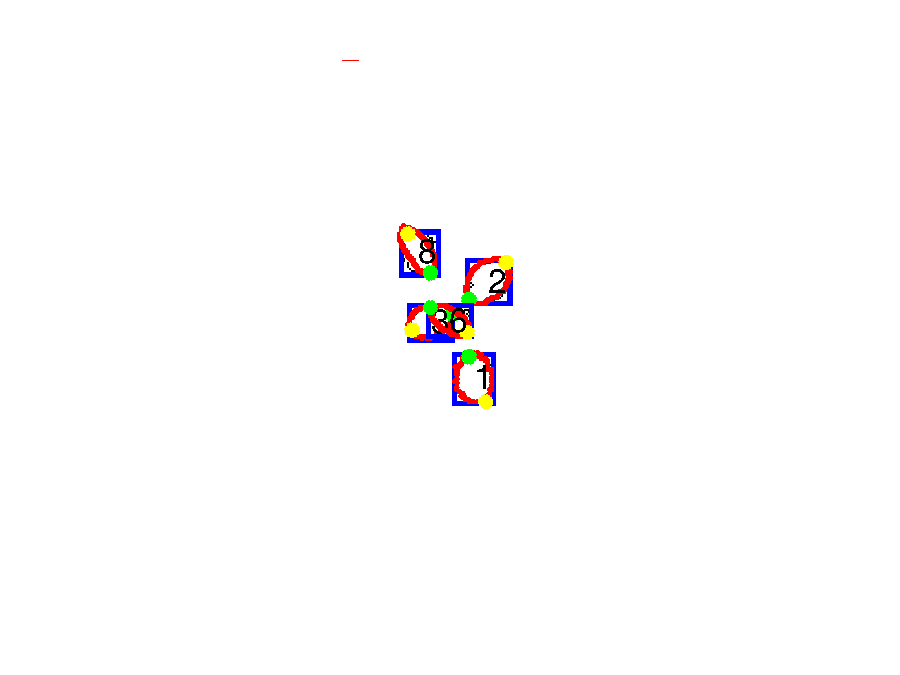
\includegraphics[trim= 100 70 120 10, clip, width=.1\textwidth]{Figures/trackExample/3_1.pdf}&
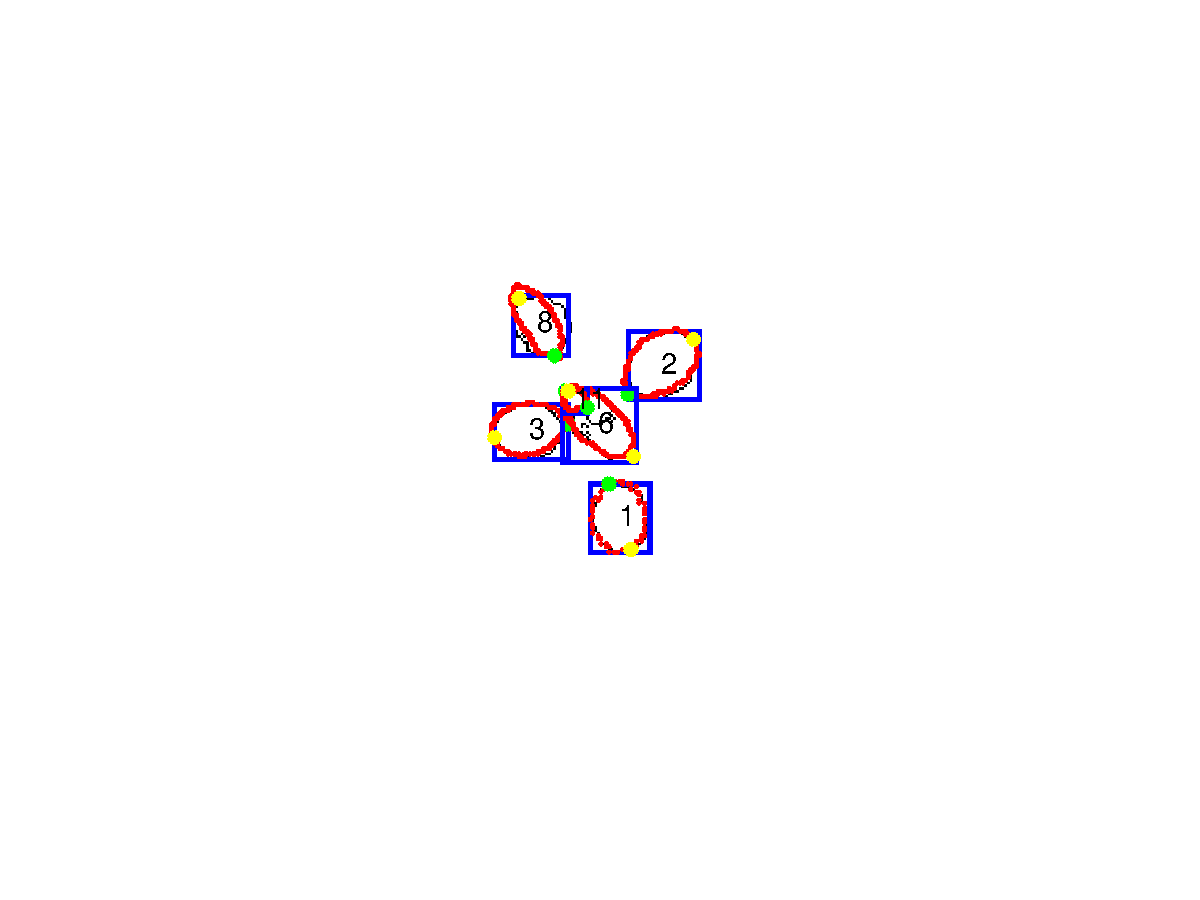
\includegraphics[trim= 100 70 120 10, clip, width=.1\textwidth]{Figures/trackExample/3_2.pdf}&
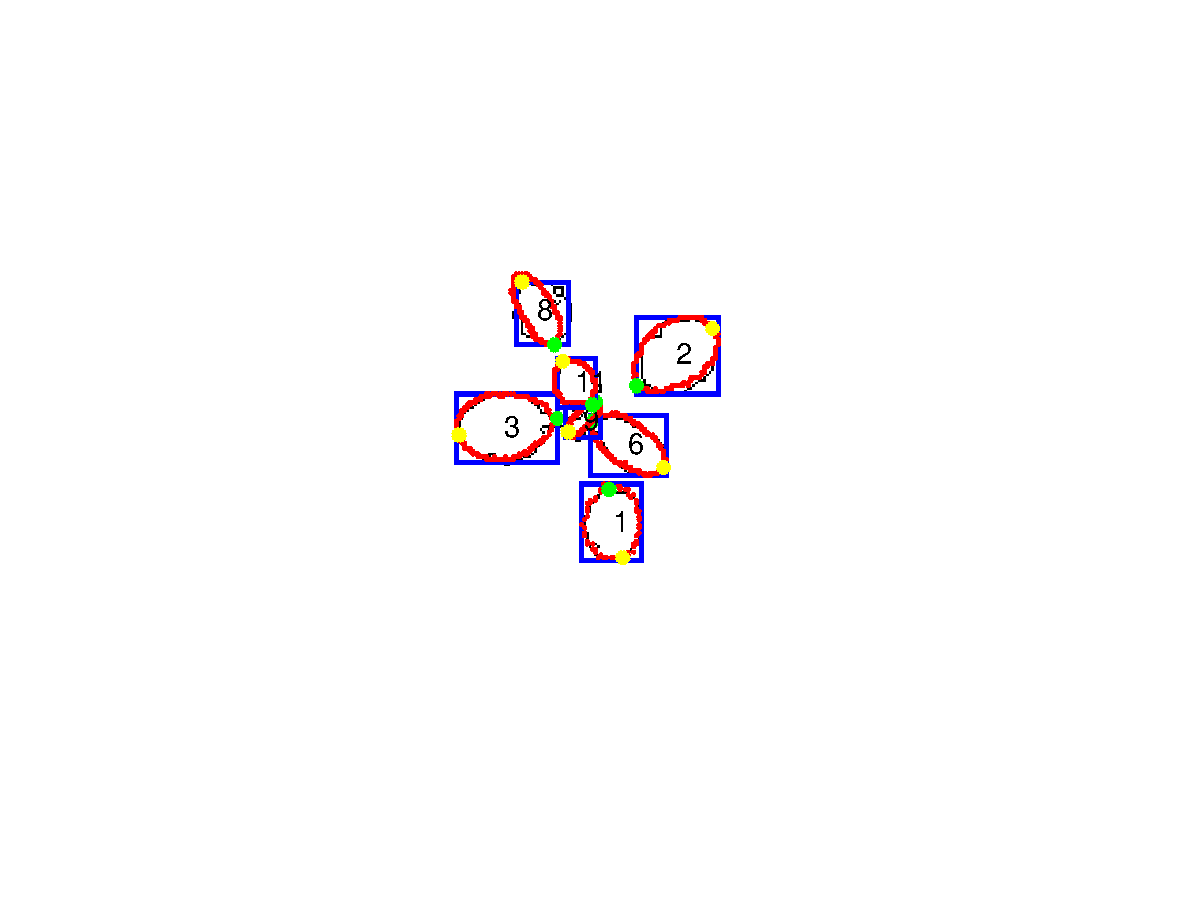
\includegraphics[trim= 100 70 120 10, clip, width=.1\textwidth]{Figures/trackExample/3_3.pdf}&
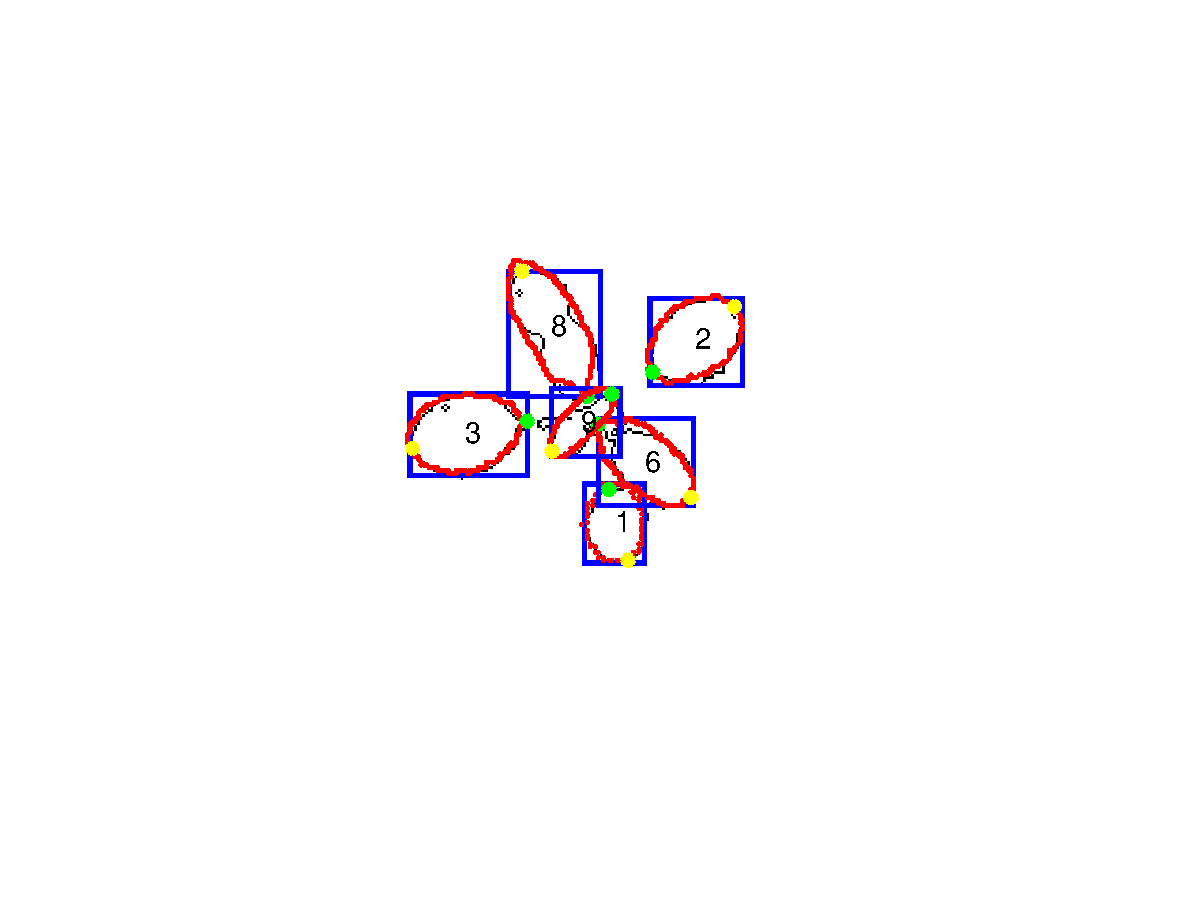
\includegraphics[trim= 100 70 120 10, clip, width=.1\textwidth]{Figures/trackExample/3_4.pdf}&
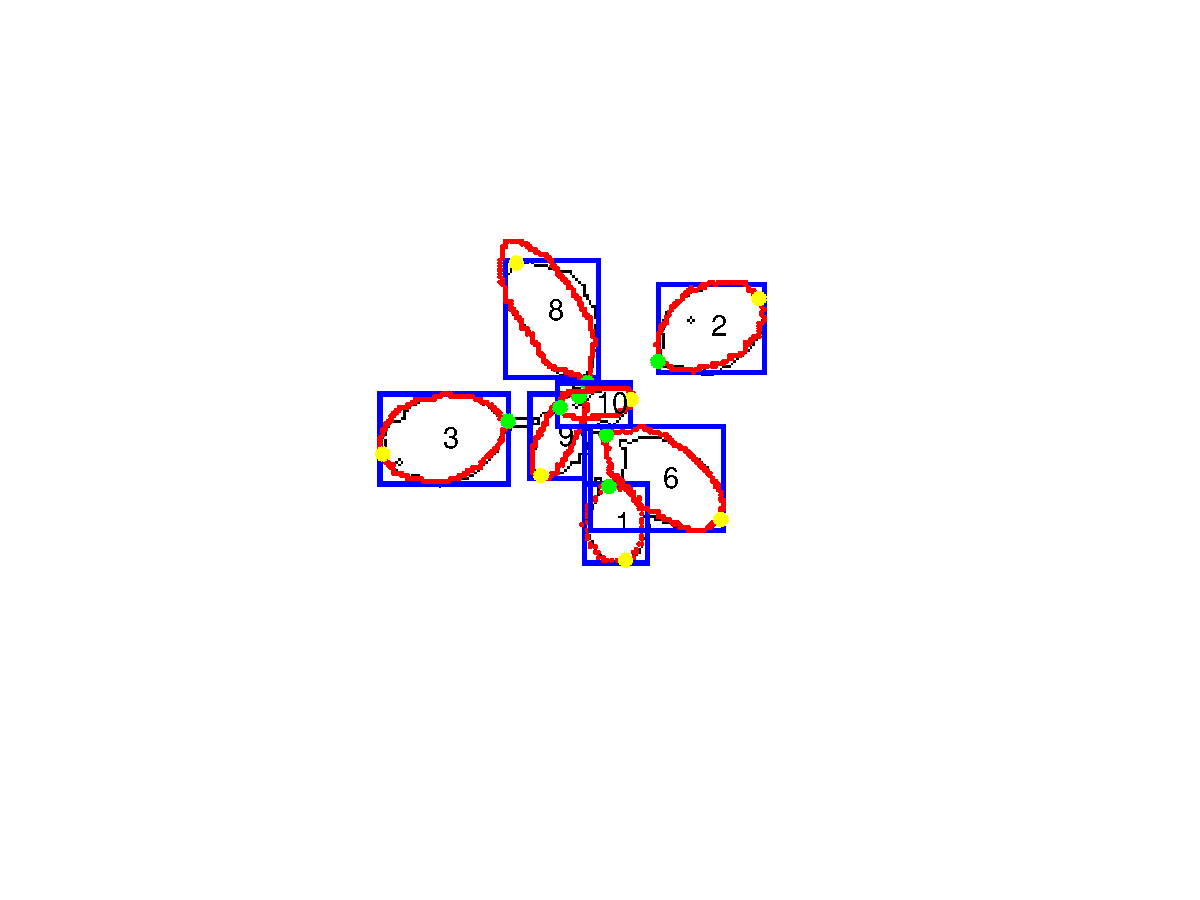
\includegraphics[trim= 100 70 120 10, clip, width=.1\textwidth]{Figures/trackExample/3_5.pdf}&
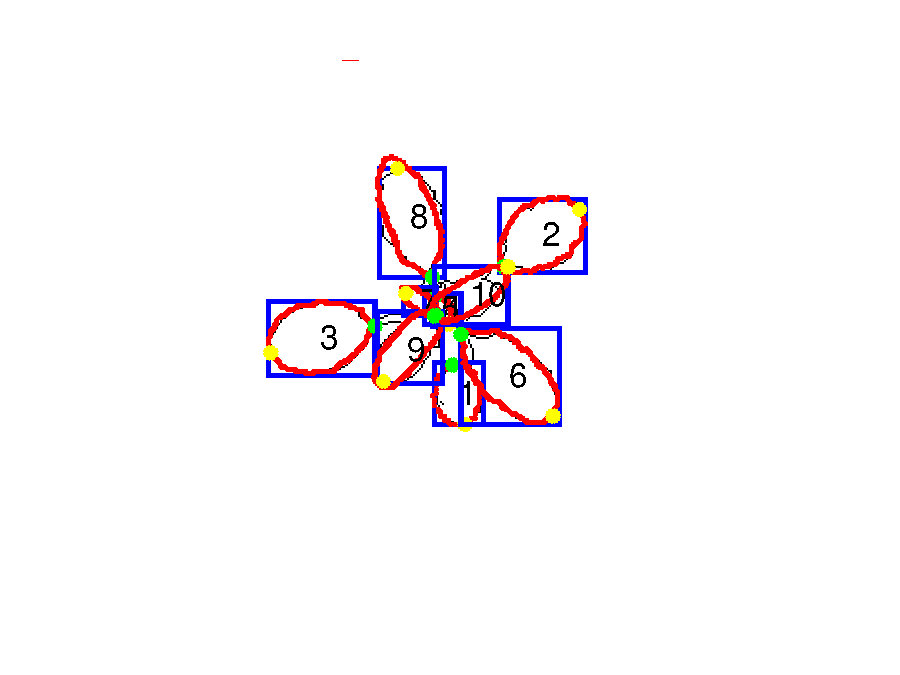
\includegraphics[trim= 100 70 120 10, clip, width=.1\textwidth]{Figures/trackExample/3_6.pdf}&
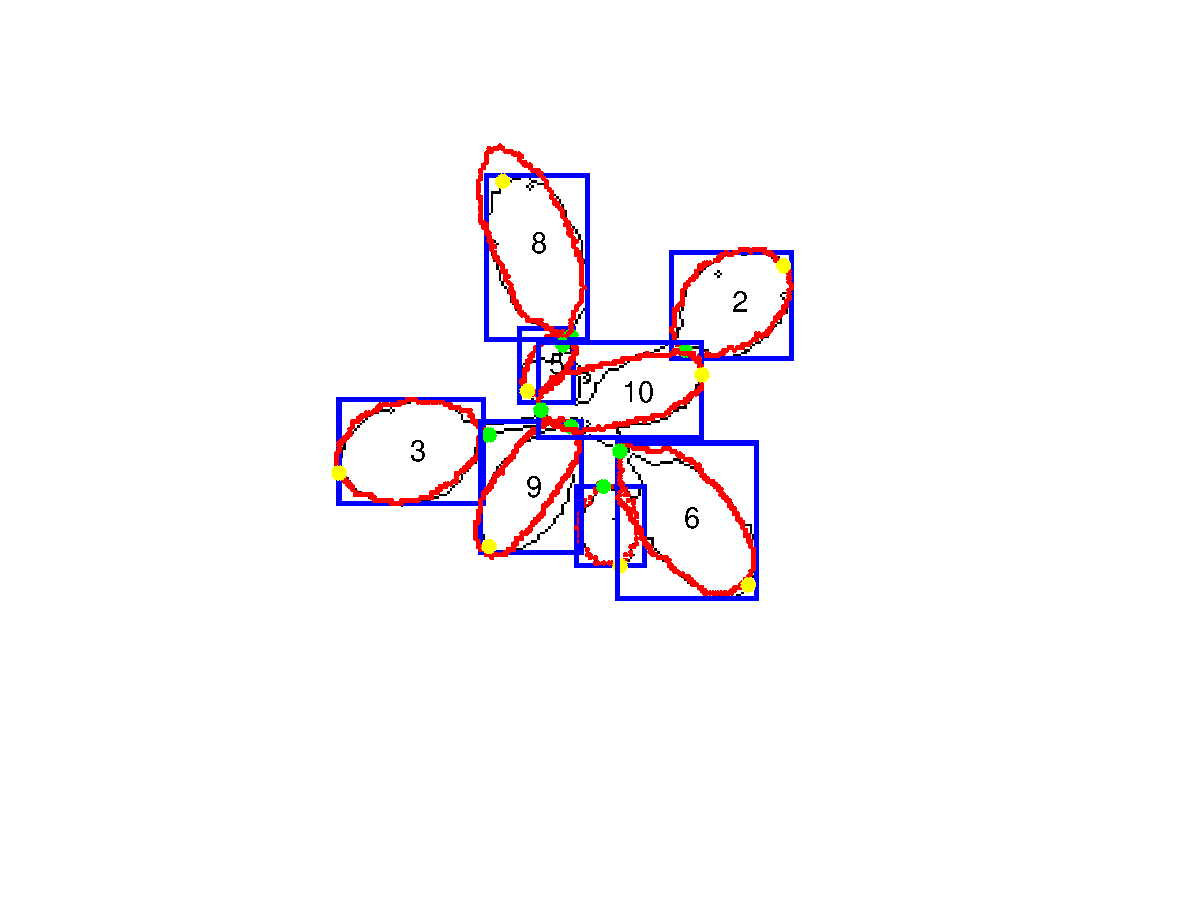
\includegraphics[trim= 100 70 120 10, clip, width=.1\textwidth]{Figures/trackExample/3_7.pdf}&
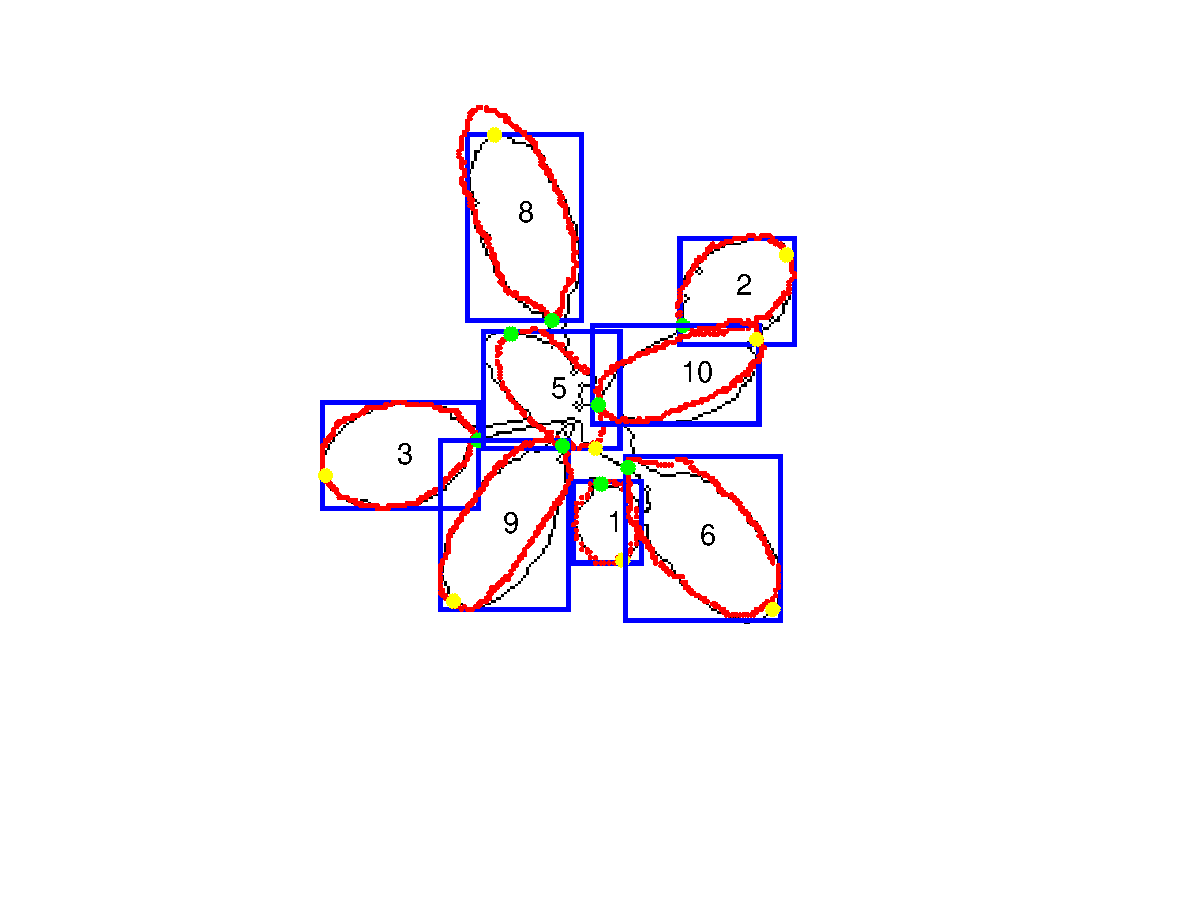
\includegraphics[trim= 100 70 120 10, clip, width=.1\textwidth]{Figures/trackExample/3_8.pdf}&
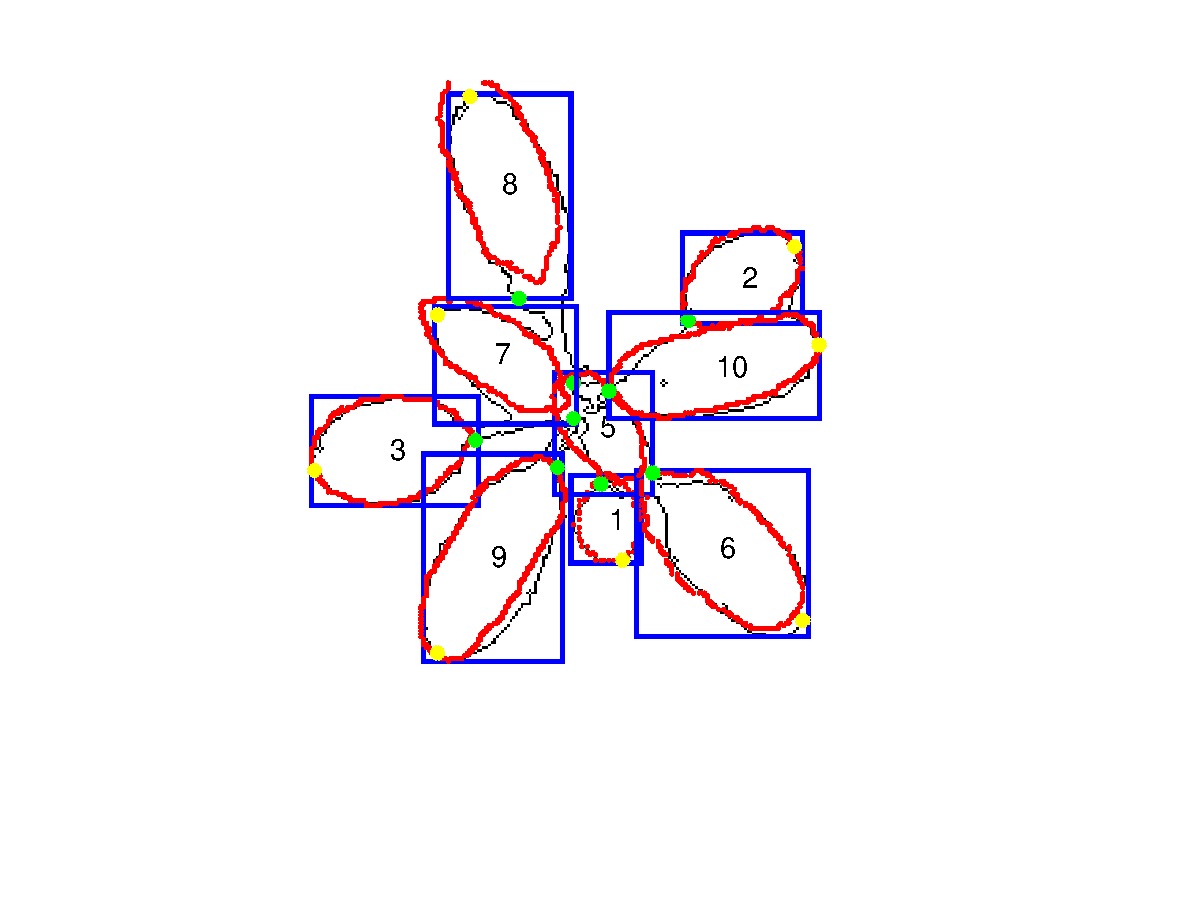
\includegraphics[trim= 100 70 120 10, clip, width=.1\textwidth]{Figures/trackExample/3_9.pdf}\\

& Day 1 & Day 2 & Day 3 & Day 4 & Day 5 & Day 6 & Day 7 & Day 8 & Day 9 \\
\end{tabular}
\caption{Tracking result for one video with one frame for each day. $(a)$ Example frames in the video. $(b)$ Leaf label results overlaid with tip locations. $(c)$ Leaf tracking results. }
\label{fig:trackExample}
\end{centering}
\end{figure*}


\begin{figure*}
\centering
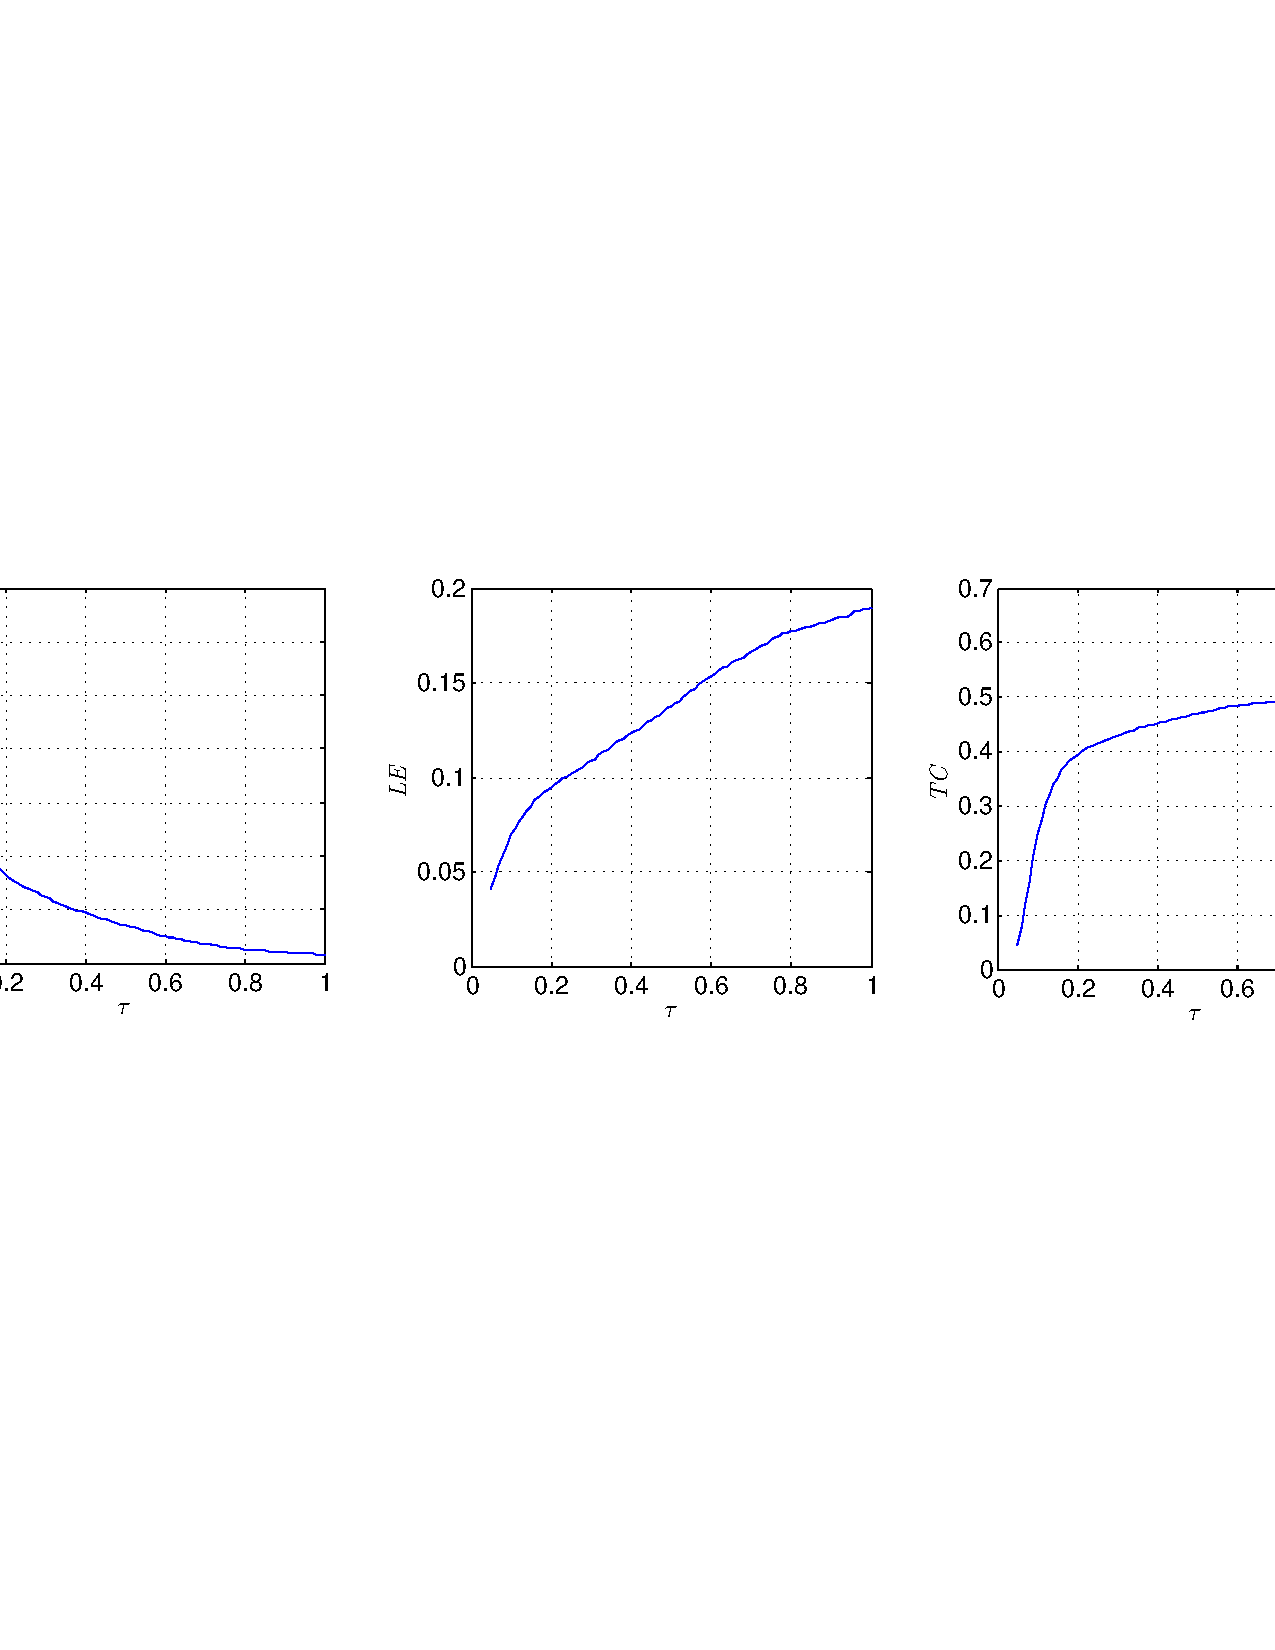
\includegraphics[width=.81\textwidth]{Figures/performance.pdf}\\
\caption{Performance of the baseline method on the testing set of the fluorescence modality of Arabidopsis plant.}
\label{fig:performance}
\end{figure*}


\subsection{Performance and Analysis}
We apply our algorithm to all $144$ frames of each video and evaluate the performance on labeled $36$ frames.
Leaf alignment is applied to the last frame of each video.
Figure~\ref{fig:alignResult} shows some examples of leaf alignment results.
Our framework works very well on segmenting large leaves with no overlap to neighbor leaves.
For overlapping leaves, it becomes more challenging as the edges in the overlapping area are more difficult to be detected.
However, when the overlapping leaves are further away from the center, they will have a higher chance to be detected as shown in $(c)$ of Figure~\ref{fig:alignResult}.
When the overlapping leaves are close to the center, smaller leaves will be covered by larger leaves as shown in $(a), (d), (e)$ of Figure~\ref{fig:alignResult}.


Leaf alignment provides the leaf candidates for tracking over time.
Figure~\ref{fig:trackExample} shows the leaf tracking result of one video.
The leaf template transformation works well for most of the leaves.
As plant grows, younger leaves may grow faster than older leaves and occlude the older leaves.
As shown in Figure~\ref{fig:trackExample} (b), purple leaf replaces the red leaf at day $6$.
Our backward tracking algorithm tracks leaves from the last frame to the first frame.
The two leaves are still being considered as one leaf (ID $8$) in day $4$ and day $3$.
Leaf $8$ in day $1$ and $2$ is a leaf ID switch w.r.t.~the purple ground truth leaf and will not be considered as a consistently tracked leaf.
However, they are still evaluated as well aligned and segmented leaves.
%Leaves will be deleted when it becomes small and the leaf underneath it will be detected.


For quantitative evaluation, we vary $\tau$ from $0$ to $1$ and generate the first three evaluation metrics, as shown in Figure~\ref{fig:performance}.
{\it{ULR}} decreases as $\tau$ increases as more leaves are being considered as matched leaves.
As $\tau$ keeps increasing, {\it{ULR}} approaches a constant value, which is the different number in leaf counting that results from both miss detection and false alarms.
{\it{LE}} increases as $\tau$ increases as it includes leaves with larger tip-based errors for averaging.
{\it{TC}} increases as $\tau$ increases as more leaves are being considered as correctly tracked leaves.
Note that {\it{TC}} is influenced by the length of frames evaluated for each video.
As the longer frames we evaluate, the higher chance tracking will fail.
Overall, our method can detect $87\%$ and track $50\%$ of all labeled leaves with less than $20\%$ average tip-based errors.

We generate a label image for each frame based on the leaf segmentation results and compute the {\it{SBD}} score for each labeled image.
The average {\it{SBD}} over all images is $0.61$.









